%%% Newden Repository %%%
%%% By: Paulo Vitor Correia de Oliveira %%%
\documentclass[11pt, a4paper]{article}
\usepackage{denplate}

%%% ===== Metadata ===== %%%
\title{Álgebra Linear}
\author{Repositório NewDen}
\date{}

\begin{document}
\maketitle
\void[-3]

\lin
\void[-1]
\tableofcontents
\lin
\newpage

\section{Conceitos Elementares}

Álgebra Linear é o estudo de coisas que se comportam com linearidade, em especial com o uso de vetores, matrizes, transformações lineares e temas tangentes a isso. De início, o que precisamos é o conhecimento geral sobre esses conceitos e relações entre eles.

\subsection{Espaços Vetoriais}

O nosso principal objeto de estudo na álgebra linear é o \textbf{vetor}, e sua definição é: Um vetor é um elemento de um espaço vetorial. Note que essa definição não nos ajuda muito, pois ela se apoia em uma outra definição ainda desconhecida: um espaço vetorial. Por sorte, esse possui uma definição mais convincente.

Um \textbf{espaço vetorial} é um espaço \(V\) equipado de duas operações soma e produto por escalar \((+,\cdot)\), onde \(+:V\times V \rightarrow V\) e \(\cdot : \Real \times V \rightarrow V\) onde valem todas as oito propriedades a seguir:

\begin{enumerate}
    \item \textbf{Comutatividade da soma: \(u,v\in V \rightarrow u+v=v+u\)}

    \item \textbf{Associatividade da soma: \(u,v,w\in V \rightarrow (u+v)+w=u+(v+w)\)}

    \item \textbf{Elemento neutro da soma: \(\exists 0\in V\) t.q. \(u \in V \rightarrow u+0=u\)}

    \item \textbf{Inverso aditivo: \(u\in V \rightarrow \exists(-u)\in V\) t.q. \(u+(-u)=0\)}

    \item \textbf{Distributividade da soma: \(u,v\in V, \alpha \in \Real \rightarrow \alpha(u+v)=\alpha u+\alpha v\)}

    \item \textbf{Distributividade do produto por escalar: \(u\in V,\alpha, \beta \in \Real \rightarrow (\alpha + \beta)u=\alpha u + \beta u\)}

    \item \textbf{Associatividade do produto por escalar: \(u\in V,\alpha,\beta\in V \rightarrow \alpha(\beta u)=(\alpha \beta)u\)}

    \item \textbf{Elemento neutro do produto: \(u\in V \rightarrow 1\cdot u=u\)}
\end{enumerate}

Note que no fundo, essas propriedades significam: um espaço vetorial é um espaço que a soma e produto são bem comportadas e lineares. Além disso, podemos fazer mais algumas definições: Se \(V\) é um espaço tal que \((V,+,\cdot)\) é um espaço vetorial e \(W\subset V\), então \((W,+,\cdot)\) também é um espaço vetorial e é um \textbf{subespaço vetorial} de \(V\).

Note que \(\Real^n\) é um espaço vetorial. Além disso, se \(v \in \Real^n\), podemos tratá-lo como uma lista de números \(v=(v_1,...,v_n)\), onde a soma e produto são feitos coordenada a coordenada, assim como a igualdade e conceitos similares. Também podemos desenhar um vetor \(v\) no \(\Real^n\) como uma seta indo da origem ao ponto de coordenadas \((v_1,...,v_n)\).

Veremos que essa representação tem um significado mais profundo do que parece, e não só para o \(\Real^n\), mas só um pouco mais a frente.

Podemos definir mais algumas operações muito relevantes para lidar com vetores:

\begin{itemize}
    \item \textbf{Norma euclidiana}: \(||v||_2=\sqrt{v_1^2+v_2^2+...+v_n^2}\)
    \item \textbf{Produto escalar}: \( \displaystyle \langle v,w \rangle=\sum_{i=1}^{n}v_iw_i\)
\end{itemize}

Esses operadores possui muitas propriedades importantes e/ou interessantes, como \(\langle a,b\rangle =||a||_2\cdot ||b||_2 \cdot cos(\theta)\), onde \(\theta\) é o ângulo entre os dois vetores no \(\Real^n\). Se representarmos os dois vetores \(a,b\) no espaço desenhando o ângulo entre eles, teremos o seguinte desenho:

\begin{center}
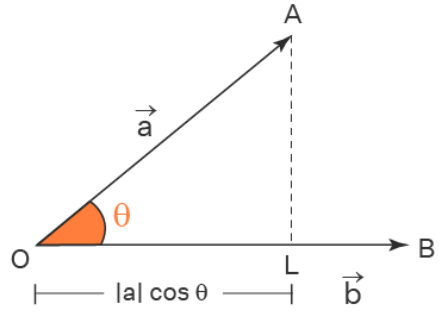
\includegraphics[width=16em]{Imagens/vectors.png}
\end{center}

Nele, veja que podemos aplicar o teorema de Pitágoras e concluir que \(AL^2=OA^2-LO^2\) e também que \(AL^2+LB^2=BA^2\). Como \(OA=||a||_2\), podemos usar trigonometria para concluir que \(AL=||a||_2 \cdot sen(\theta)\) e \(LO=||a||_2 \cdot cos(\theta)\), e então, \(LB=||b||_2 - ||a||_2 \cdot cos(\theta)\). Além disso, \(BA=||b-a||_2\). Com isso, podemos aplicar o teorema de Pitágoras do triângulo \(ALB\), concluindo:

\[||a||_2^2\cdot sen^2(\theta) +||b||_2^2 + ||a||_2^2\cdot cos^2(\theta)-2||a||_2||b||_2\cdot cos(\theta)=||b-a||_2^2\]

Que pode ser simplificada para:

\[||a||_2^2 +||b||_2^2 -2||a||_2||b||_2\cdot cos(\theta)=||b-a||_2^2\]

Além disso, note que:

\[||b-a||_2^2=\sum_{i=1}^{n}{(b_i-a_i)^2}=||b||_2^2+||a||_2^2-2\langle a,b \rangle\]

E igualando as duas expressões, podemos concluir que:

\[\langle a,b \rangle = ||a||_2 \cdot ||b||_2 \cdot cos(\theta)\]

Esse desenho também nos diz um pouco sobre a \textbf{projeção} de um vetor sobre o outro: o segmento \(LO\) é a projeção de \(a\) sobre \(b\), que pode ser interpretada como a sombra que um vetor faz sobre o outro, mas teremos mais tempo para explorar isso mais a frente.

Vamos agora falar um pouco mais de subespaços. Sabemos a definição de subespaços, mas como eles se comportam no geral? Vamos pensar em alguns exemplos do que são e o que não são subespaços:

\begin{itemize}
    \item Seja \(E\) o espaço vetorial das funções reais de uma variável (veja que ele cumpre as propriedades). O subconjunto \(C^{k}\) das funções \(k\) vezes diferenciáveis é um subespaço vetorial de \(E\), assim como o subconjunto \(C^{\infty}\), da funções infinitamente diferenciáveis.

    \item Seja \(P\) o espaço dos polinômio de grau menor ou igual a \(m\). Veja que o espaço dos polinômios de grau exatamente \(m\) não é subespaço dele, pois dois polinômios de grau \(m\) somados podem formar um polinômio de grau menor, que sai do espaço definido.

    \item Seja \(F\) um espaço vetorial que tem um vetor \(v\). Então, o conjunto dos múltiplos de \(v\) também é um subespaço vetorial de \(F\).
\end{itemize}

Então podemos ver que nem todo exemplo de parte intuitiva de um espaço vetorial forma um subespaço vetorial, mas no geral, temos bons subespaços vetoriais para analisar.

Seja \(E\) um espaço vetorial e \(F_1,F_2\) subespaços vetoriais de \(E\). Se \(F_1 \cap F_2=\{0\},\) representamos a união dos subespaços \(F_1+F_2\) como \(F_1 \oplus F_2\), e isso é chamado de \textbf{soma direta} de \(F_1\) e \(F_2\). 

Dito isso, dizer que \(F=F_1 \oplus F_2\) é equivalente a dizer que \(\forall w\in F,\) podemos escrever \(w\) de forma única como \(w=v_1+v_2\), onde \(v_1\in F_1\) e \(v_2 \in F_2\). Para demonstrar isso, note que:

\begin{itemize}
    \item \(F=F_1 \oplus F_2 \rightarrow\) \(F_1 \cap F_2=\{0\}\). Além disso, suponha que exista \(w=v_1+v_2=u_1+u_2\), onde \(u_1,v_1\in F_1\) e \(u_2,v_2 \in F_2\). Então, \(x=v_1-u_1=u_2-v_2\). Note que \(u_1-v_1\in F_1\) e também \(u_2-v_2 \in F_2\), logo, \(x \in F_1 \cap F_2\), portanto, \(x=0\). Isso mostra que só há uma forma de escrevermos \(w\).

    \item Se só há uma forma de escrevermos \(w=v_1+v_2\) para qualquer \(w\), tome \(w \in F_1 \cap F_2\). Note que \(w=w+0=0+w\), onde \(w,0\in F_1\) e \(0,w \in F_2\). Pela unicidade, devemos ter \(0=w\), mostrando então que \(F=F_1 \oplus F_2\) pois \(F_1 \cap F_2 = \{0\}\).
\end{itemize}

Note que com isso, podemos aplicar esse resultado para várias coisas, onde uma delas é que dividir o \(\Real^n\) em hiperplanos que só se intersectam em um ponto forma uma soma direta. Um exemplo de divisão é dividir ele nas retas que tem uma das coordenadas variável e as restantes fixas iguais a zero: é fácil ver que só há uma forma de construir um vetor como soma dos vetores em outros subespaços, pois cada subespaço é responsável por alterar uma coordenada.

\subsection{Matrizes}

Agora, veremos outro elemento crucial do estudo de vetores: as \textbf{matrizes}. Uma matriz é graficamente uma tabela \(N\times M\), com \(N\) linhas e \(M\) colunas. No geral, uma matriz também pode ser vista como uma junção de \(M\) vetores coluna, e essa interpretação também nos ajuda em muitas contas.

Podemos fazer operações com matrizes: a \textbf{soma}, que é feita entrada a entrada correspondente e também a \textbf{multiplicação por escalar}, novamente, feita entrada a entrada. Veja que essas operações são análogas as operações vetoriais, justamente pois matrizes e vetores estão fortemente relacionados.

Além dessas operações, também há uma operação exclusiva de matrizes: a \textbf{multiplicação de matrizes}. Para duas matrizes \(A \in \Real^{N \times M}, B \in \Real^{P \times Q}\) serem multiplicáveis, devemos ter \(M=P\), e o resultado será uma matriz \(N \times Q\) onde podemos calcular as entradas da matriz produto \(AB\) com a expressão \(\displaystyle AB_{ij}=\sum_{k=1}^{M}A_{ik}B_{kj}\). Segue um exemplo de multiplicação de matrizes (verifique).

\[
\begin{bmatrix}
1 & 2\\
2 & 3\\
\end{bmatrix}
\times
\begin{bmatrix}
1 & 0\\
0 & 2\\
\end{bmatrix}
=
\begin{bmatrix}
1 & 4\\
2 & 6\\
\end{bmatrix}
\]

Além disso tudo, seja \(X = \{v_1, v_2, \ldots, v_n\}\) um conjunto de \(n\) vetores de um espaço vetorial \(V\) e \(Y = \{\alpha_1, \alpha_2, \ldots, \alpha_n\}\) um conjunto de escalares. A expressão \(\alpha_1 v_1 + \alpha_2 v_2 + \cdots + \alpha_n v_n\) é chamada de \textbf{combinação linear} de \(X\).

Indo além da multiplicação de matrizes por definição explícita, perceba que uma multiplicação de matrizes pode ser interpretada como \textbf{várias combinações lineares de vetores}.

Podemos interpretar que o \(i-\)ésimo vetor-coluna na matriz da direita são os coeficientes que devemos multiplicar cada vetor coluna da matriz da esquerda para que a soma desses vetores coluna multiplicados pelos coeficientes seja o \(i-\)ésimo vetor coluna da matriz final.

Da mesma forma, podemos interpretar que a \(i-\)ésima linha da matriz da esquerda representa os coeficientes dos vetores-linha da matriz da direita para que a combinação linear deles seja o \(i-\)ésimo vetor-linha da matriz resultado. Lembre-se muito bem dessas duas interpretações, pois serão muito valiosas mais a frente.

A multiplicação de matrizes é uma operação associativa, mas não é comutativa: \(A(BC)=(AB)C\), mas \(AB \ne BA\). Prove a associatividade e dê um contra exemplo para a não comutatividade.

Há ainda uma outra definição que, por ora não será muito usada, mas tem grande relevância no estudo das equações diferenciais: a \textbf{exponencial de matriz}. Ela é definida com o mesmo formato da série de Taylor da exponencial, mas cujos termos \(x^k\) são as potências de matrizes \(A^k\), onde uma potência de matriz é definida como uma sequência de multiplicações de matriz. No geral, a formula da exponencial de matriz é: \(e^A=\displaystyle\sum_{n=1}^{\infty}{\frac{A^n}{n!}}\).

Há ainda uma lista de definições que importam e serão vistos com muita frequência ao decorrer do documento:

\begin{itemize}
    \item \textbf{Matriz Transposta}: \(A^T\), sendo a matriz obtida ao trocarmos as linhas de \(A\) por suas colunas, isto é, \(A_{ij}=A^T_{ji}\). Uma matriz é \textbf{simétrica} se \(A=A^T\).

    \item \textbf{Matriz Conjugada}: \(\overline{A}\), onde a operação feita é tomar o conjugado complexo de todas as entradas da matriz caso ela seja uma matriz de números complexos, mantendo as dimensões da matriz.

    \item \textbf{Matriz Transposta Conjugada}: \(A^*\), e essa definição é a combinação das duas definições de cima ao mesmo tempo: \(A^*=\overline{A^T}\). Uma matriz é \textbf{hermitiana} se \(A=A^*\).

    \item \textbf{Matriz Identidade}: \(I\). É uma matriz quadrada que possui todas entradas iguais a zero, exceto a diagonal que possui valores 1.

    \item \textbf{Matriz Inversa}: \(A^{-1}\), sendo essa uma matriz tal que \(AA^{-1}=A^{-1}A=I\). Uma matriz \(A_E\) é \textbf{inversa pela esquerda} de \(A\) se \(A_EA=I\), mas não necessariamente \(AA_E=I\). Da mesma forma, uma matriz \(A_D\) é \textbf{inversa pela direita} de \(A\) se \(AA_D=I\), mas não necessariamente \(A_DA=I\).

    \item \textbf{Traço de uma matriz}: \(tr(A)\), é a soma dos elementos da diagonal da matriz.
\end{itemize}

Também podemos lidar com matrizes tratando pedaços delas como \textbf{blocos}. Vamos imaginar por exemplo uma matriz \(4 \times 4\). Ela pode ser interpretada como uma matriz de \(2 \times 2\) blocos de tamanho \(2 \times 2\), da seguinte forma:

\void[-0.8]

\[
\begin{bmatrix}
a_{11} & a_{12} & b_{11} & b_{12}\\
a_{21} & a_{22} & b_{21} & b_{22}\\
c_{11} & c_{12} & d_{11} & d_{12}\\
c_{21} & c_{22} & d_{21} & d_{22}\\
\end{bmatrix}
=
\begin{bmatrix}
    A & B\\
    C & D\\
\end{bmatrix}
\]

\void[-0.4]

Esses blocos de matrizes podem ser operados como matrizes menores na multiplicação de matrizes e produzirão os mesmos resultados, desde que as dimensões das multiplicações sejam condizentes. 

Vamos pensar de uma forma generalizada para tentar verificar essa propriedade: Suponha que uma matriz \(A\) seja dividida em blocos da seguinte forma:

\void[-1]

\[
A=
\begin{bmatrix}
a_{11} & a_{12} & a_{13} & ... & a_{1m}\\
a_{21} & a_{22} & a_{23} & ... & a_{2m}\\
a_{31} & a_{32} & a_{33} & ... & a_{3m}\\
\vdots & \vdots & \vdots & \ddots & \vdots \\
a_{n1} & a_{n2} & a_{n3} & \hdots & a_{nm}
\end{bmatrix}
=
\begin{bmatrix}
B_{11} & B_{12} & ... & B_{1q}\\
B_{21} & B_{22} & ... & B_{2q}\\
\vdots & \vdots & \ddots & \vdots \\
B_{p1} & B_{p2} & \hdots & B_{pq}
\end{bmatrix}
\]

\void[-0.5]

Suponha que exista outra matriz de blocos \(C\) e queremos fazer a multiplicação de matrizes \(AC\) mas operando nos blocos, e não entrada a entrada. Para isso ser possível, veja que a multiplicação de linha e coluna de matrizes deve ser possível na escala de blocos e todo produto \(B_{ik}D_{kj}\) deve ser factível. Verificando as necessidades das dimensões das matrizes, concluímos que:

\begin{itemize}
    \item O número de linhas de blocos na matriz \(C\) deve ser igual ao número de colunas de blocos na matriz \(D\).
    \void[-0.1]
    \item O número de colunas dos blocos \(B\) na mesma coluna de blocos mas em linhas diferentes deve ser o mesmo.
    \void[-0.1]
    \item O número de linhas dos blocos \(B\) na mesma linha de blocos mas em colunas diferentes deve ser o mesmo.
    \void[-0.1]
    \item O número de linhas dos blocos \(D\) na mesma linha de blocos mas em colunas diferentes deve ser o mesmo.
    \void[-0.1]
    \item O número de colunas dos blocos \(D\) na mesma coluna de blocos mas em linhas diferentes deve ser o mesmo.
    \void[-0.1]
    \item O número de colunas dos blocos \(B\) na coluna de blocos \(k\) deve ser igual ao número de linhas dos blocos \(D\) na linha de blocos \(k\).
\end{itemize}

Note que as condições 2 até 5 implicam somente que \textbf{os blocos das duas matrizes devem estar alinhados verticalmente e horizontalmente}, e assim também será a matriz resultado. Ao cumprir essas propriedades, é possível multiplicar as matrizes. Agora, vamos olhar para o bloco \(E_{xy}\) da matriz resultado da multiplicação \(AC\), e mais especificamente para entrada qualquer \(ij\) de \(E\) que pertence ao bloco \(E_{xy}\). Sabemos que \(E_{xy}\) foi obtida por:

\void[-1]

\[\sum_{k=1}^{q}B_{xk}D_{ky}\]

\void[-0.5]

E portanto, sendo \(\alpha_{xk}\) o número de colunas de \(B_{xk}\), a entrada \(ij\) de \(E\) em \(E_{xy}\) é dada por:

\void[-1]

\[\sum_{k=1}^{q}(B_{xk}D_{ky})_{ij}=\sum_{k=1}^{q}\sum_{u=1}^{\alpha_{xk}}({B_{xk}})_{iu}\cdot(D_{kj})_{uj}\]

\void[-0.5]

Um detalhe é que, na expressão acima, \(({B_{xk}})_{iu}\) não se refere a entrada \(iu\) de \(B_{xk}\), mas sim à entrada \(i'u\), onde \(i'\) é o índice da linha de \(B_{xk}\) que corresponde a linha \(i\) da matriz completa \(E\). O mesmo está sendo considerado para \(j\) em \(D\).

Dito isso, veja que a expressão acima é completamente equivalente a multiplicar a linha \(i\) de \(A\) e a coluna \(j\) de \(C\), mostrando que para toda entrada, as duas formas de fazer essa multiplicação são equivalentes, e com isso, concluímos que representar matrizes em blocos é um método válido caso os blocos sejam \textbf{alinhados} e de dimensões \textbf{compatíveis}.

\subsection{Sistemas Lineares}

Sistemas lineares são conjuntos com equações que usam um determinado conjunto de variáveis, e resolvê-los significa encontrar valores para as variáveis que tornem as equações verdadeiras. Alguns exemplos de sistema linear são \(\{2x + y = 3,\ x + y = 4\}\), que possui duas equações e as variáveis \(x\) e \(y\), e também \(\{x + y + z = 1,\ 2x + y + z = 4,\ x + 7y + z = 7,\ 4x + 4y = 9\}\), com quatro equações e três variáveis.

Podemos representar sistemas lineares com matrizes: uma matriz contém todos os coeficientes, onde cada linha representa os coeficientes de uma equação. Essa matriz multiplica outra matriz (um vetor, que é uma matriz de uma só coluna) à sua direita: um vetor cujas entradas são as variáveis correspondentes, na mesma ordem dos coeficientes. Esse produto é igualado a outro vetor, representando os resultados das equações.

Por exemplo, os sistemas anteriores podem ser representados assim:

\void[-0.5]

\[
\begin{bmatrix}
2 & 1\\
1 & 1
\end{bmatrix}
\begin{bmatrix}
x\\
y
\end{bmatrix}
=
\begin{bmatrix}
3\\
4
\end{bmatrix}
\quad \text{e} \quad
\begin{bmatrix}
1 & 1 & 1\\
2 & 1 & 1\\
1 & 7 & 1\\
4 & 4 & 0
\end{bmatrix}
\begin{bmatrix}
x\\
y\\
z
\end{bmatrix}
=
\begin{bmatrix}
1\\
4\\
7\\
9
\end{bmatrix}
\]

Essa representação formal permite uma maneira mais eficiente de trabalhar com sistemas. Mas será que ela também nos ajuda a resolvê-los?

No geral, existe sim uma forma generalizada de resolver sistemas lineares a partir da representação por matrizes. Trata-se de um algoritmo chamado \textbf{Eliminação Gaussiana}, que permite fazer inferências sobre as soluções de um sistema linear. Um sistema pode ter nenhuma, uma ou infinitas soluções - pois se houver duas, há infinitas combinações lineares entre elas que também são soluções.

O algoritmo consiste em aplicar operações que não alteram as soluções do sistema, com o objetivo de transformar a matriz \(A\) em uma matriz triangular superior, que pode ser resolvida facilmente com retrossubstituição. Uma matriz triangular superior é aquela cujos elementos abaixo da diagonal principal são todos zero.

Um sistema linear pode ser representado como \(Ax = y\), onde \(A\) é a matriz dos coeficientes, \(x\) o vetor de variáveis e \(y\) o vetor dos resultados, por exemplo:

\[
\begin{bmatrix}
1 & 2 & 3\\
2 & 1 & 3\\
4 & 5 & 6
\end{bmatrix}
\begin{bmatrix}
x\\
y\\
z
\end{bmatrix}
=
\begin{bmatrix}
1\\
2\\
3
\end{bmatrix}
\]

As operações devem ser aplicadas tanto à matriz \(A\) quanto ao vetor \(y\), mas não ao vetor de variáveis. As operações válidas são:

\begin{itemize}
    \item \(M(i, \alpha)\): multiplicar a linha \(i\) por um escalar \(\alpha \ne 0\).
    \item \(P(i,j)\): trocar as linhas \(i\) e \(j\) de posição.
    \item \(S(i, \alpha, j)\): somar \(\alpha\) vezes a linha \(j\) à linha \(i\).
\end{itemize}

Essas operações preservam o conjunto de soluções do sistema:

\begin{itemize}
    \item Em \(M(i, \alpha)\), como multiplicamos ambos os lados da equação por \(\alpha\), as soluções se mantêm.
    \item Em \(P(i, j)\), apenas trocamos a ordem das equações.
    \item Em \(S(i, \alpha, j)\), se uma solução resolve as equações \(i\) e \(j\), também resolve a nova linha \(i\).
\end{itemize}

Portanto, nenhuma solução é perdida com essas operações. O algoritmo então consiste em, começando da linha 1 e coluna 1, seguir os seguintes passos:

\begin{enumerate}
    \item Se todos os valores da coluna forem zero, passe para a próxima coluna.
    \item Caso contrário, mova uma linha com um valor diferente de zero para a linha atual, torne o valor 1 multiplicando a linha por um escalar e subtraia múltiplos dessa linha das demais linhas para zerar o restante da coluna.
    \item Avance para a próxima linha e coluna, repetindo o processo.
\end{enumerate}

Ao final, obtemos uma matriz triangular superior, e podemos resolver o sistema por \textbf{retrossubstituição}. A matriz resultante é chamada de \textbf{matriz escalonada}. Os primeiros elementos não nulos de cada linha são chamados de \textbf{pivôs}, e suas colunas de \textbf{colunas pivô}. O número total de pivôs é chamado de \textbf{posto} da matriz, que também é o número de colunas linearmente independentes.

O posto de uma matriz é o número de colunas linearmente independentes de \(A\).

Dado que a Eliminação Gaussiana transforma um sistema \(Ax = b\) em outro equivalente \(Ux = c\), podemos estudar as soluções observando \(U\) e \(c\). As possíveis situações são:

\begin{itemize}
    \item Se uma linha de \(U\) for composta apenas por zeros e o valor correspondente de \(c\) for diferente de zero, o sistema não tem solução.
    \item Se uma linha de \(U\) for composta por zeros e o valor de \(c\) também for zero, a equação é redundante.
    \item Se alguma coluna de \(U\) não tiver pivô (isto é, o número de pivôs for menor que o número de variáveis), então o sistema tem \textbf{infinitas soluções}, pois existe uma variável livre.
    \item Se todas as colunas tiverem pivôs, então o sistema tem uma \textbf{única solução}, obtida por retrossubstituição.
\end{itemize}

Portanto, a Eliminação Gaussiana não apenas nos permite resolver sistemas lineares, mas também entender a estrutura de suas soluções. Logo a frente, veremos que essa abordagem matricial nos dá ferramentas poderosas que vão além da resolução de sistemas, nos levando a resultados importantes sobre a natureza das próprias matrizes.

\subsection{Decomposição LU}

Vimos que o algoritmo de Eliminação Gaussiana, mas não conseguimos obter de fato um método reutilizável: para todo sistema linear, temos que refazer todo o algoritmo, mesmo que mudemos apenas algo simples como o vetor \(b\). Além disso, esse método não nos dá objetos úteis que sabemos trabalhar em álgebra linear, como vetores ou matrizes. Veremos agora uma variação mais abrangente desse algoritmo que resolve esses problemas.

Podemos interpretar as três operações descritas anteriormente como matrizes, que chamaremos de \textbf{matrizes elementares}. Por exemplo, para \(m=n=5,i=4,j=2,\) temos as matrizes:

\void[-2]

\[
P(i,j)=
\begin{bmatrix}
    1&&&&\\
    &&&1&\\
    &&1&&\\
    &1&&&\\
    &&&&1\\
\end{bmatrix}
\tb[1]M(i,\alpha)=
\begin{bmatrix}
    1&&&&\\
    &1&&&\\
    &&1&&\\
    &&&\alpha&\\
    &&&&1\\
\end{bmatrix}
\tb[1]S(i,\alpha,j)=
\begin{bmatrix}
    1&&&&\\
    &1&&&\\
    &&1&&\\
    &\alpha&&1&\\
    &&&&1\\
\end{bmatrix}
\]

No geral, a estrutura dessas operações como matrizes é:

\begin{itemize}
    \item A \textbf{matriz elementar de permutação} \(E_P(i,j)\) é uma matriz identidade \(n\times n\) com as linhas \(i,j\) trocadas.
    \item A \textbf{matriz elementar de multiplicação} \(E_M(i,\alpha)\) é uma matriz identidade com a entrada \(i\) da diagonal tendo o valor \(\alpha\).
    \item A \textbf{matriz elementar de soma de linha} \(E_S(i,\alpha,j)\) é uma matriz identidade com a entrada da linha \(i\) coluna \(j\) igual a \(\alpha\).
\end{itemize}

Todas essas operações são conceitualmente invertíveis, o que nos induz a pensar que as matrizes também possuem uma inversa. E de fato, esse é o caso:

\begin{itemize}
    \item A \textbf{matriz inversa elementar de permutação} \(L_P(i,j)\) é uma matriz identidade \(n\times n\) com as linhas \(i,j\) trocadas.
    \item A \textbf{matriz inversa elementar de multiplicação} \(L_M(i,\alpha)\) é uma matriz identidade com a entrada \(i\) da diagonal tendo o valor \(1/\alpha\).
    \item A \textbf{matriz inversa elementar de soma de linha} \(L_S(i,\alpha,j)\) é uma matriz identidade com a entrada da linha \(i\) coluna \(j\) igual a \(-\alpha\).
\end{itemize}

Note então que poderíamos agora descrever nosso algoritmo de Eliminação Gaussiana como uma grande multiplicação de matrizes:

\void[-1.5]

\[Ax=b \rightarrow E_k...E_2E_1Ax=E_k...E_2E_1b\]

\void[-0.6]

E com isso, podemos descrever nosso algoritmo de decomposição LU. Para cada uma das linhas de \(A\), sua \textbf{posição} é o número de linhas que estão acima dessa linha, e seu índice é uma constante definida como sua posição inicial na matriz \(A\), sem alterações. O mesmo vale para as colunas, mas com a primeira variação do algoritmo que faremos, seu índice é sempre igual a sua posição.

Considere \(V_E\) como um conjunto ordenado que guardará operações de multiplicação e soma utilizadas, enquanto \(V_P\) guardará as operações de permutação utilizadas, ou seja, toda vez que usarmos uma operação, ela será adicionada em algum dos conjuntos. 

Definimos também que as linhas e colunas podem estar \textbf{livres} ou \textbf{ocupadas}. Inicialmente, todas as linhas e colunas estão livres.

Agora, repetimos o seguinte processo, até encerrarmos o algoritmo:

\begin{enumerate}
    \item Suponha que estamos na iteração \(i\). Seja \(j\) o menor índice de uma coluna livre que não tenha todas as suas linhas livres com valor 0. Defina que toda coluna de índice menor que \(j\) agora está ocupada. Se não existir \(j\), então encerramos o algoritmo.
    \void[0.2]
    \item Seja \(l\) o índice da linha livre que possui o valor máximo na coluna \(j\). Se não existir linha livre, então encerramos o algoritmo. Agora, usamos (ou não) uma operação de permutação para permutar a linha de índice \(l\) com a linha na posição \(i\).
    \void[0.2]
    \item Para todas as outras linhas que possuam um valor na coluna \(j\) diferente de zero, usaremos operações de soma com a linha de índice \(l\) para zerar essas linhas na coluna \(j\). Após essas operações, nossa coluna \(j\) tem um único pivô, e caso necessário, podemos usar uma operação de multiplicação para torná-lo com valor \(1\).
    \void[0.2]
    \item Após finalizarmos o algoritmo, o \(k-\)ésimo pivô está na linha \(k\), e portanto, nossa matriz resultante (que chamaremos de \(U\)) é uma matriz triangular superior. Agora, considere \(P\) inicialmente como uma matriz identidade e para cada uma das operações de permutação \(P_i\) em \(V_P\), multiplique \(P\) por \(P_i\) pela esquerda, obtendo nossa matriz \(P\) final.
    \void[0.2]
    \item Assim, considere a nossa matriz \(U_0=PA\). Agora, para todas as operações \(O_i\) de \(V_E\), considere como \(E_i\) a matriz equivalente a operação \(O_i\), considerando a posição de cada linha de índice \(k\) como a sua posição em \(U_0\). Seja \(E=E_q...E_2E_2I\). Como todas as matrizes que compõem \(E\) possuem inversa, então \(E\) possui inversa, que chamaremos de \(L=L_1L_2...L_q\).
    \void[0.2]
    \item Note que como guardamos nossas operações em \(V_E\) considerando os índices das linhas, então para qualquer permutação inicial da matriz \(A\), aplicar a matriz \(E\) chegará ao menos a uma permutação de diferença da nossa matriz U, e como nossa matriz de permutação \(P\) consiste das mesmas permutações feitas durante o nosso processo para gerar \(U\), então \(EPA=U\). Usando que \(L\) é inversa de \(E\), podemos ainda multiplicar por \(L\) pela esquerda e obtemos \(PA=LU\), que é nosso resultado final.
    \void[0.2]
    \item Pela nossa estratégia de usar o maior valor como pivô, também garantimos estabilidade numérica, e essa técnica é chamada de \textbf{pivoteamento parcial}.
    \void[0.2]
\end{enumerate}

Assim, temos que esse algoritmo prova o seguinte teorema:

\void[0.3]

\textbf{Teorema (Decomposição Lower-Upper)}: Seja \(A^{m\times n}\) uma matriz qualquer. Existem matrizes \(P,L,U\) satisfazendo as seguintes propriedades:

\begin{itemize}
    \item \(P^{m \times m}\) é uma matriz de permutação.
    \void[0.2]
    \item \(L^{m \times m}\) é uma matriz triangular inferior com entradas binárias na diagonal.
    \void[0.2]
    \item \(U^{m \times n}\) é uma matriz triangular superior.
\end{itemize}

E além disso, vale que \(PA=LU\).

\void[0.6]

O teorema também funciona caso passarmos a condição de \(L\) ter entradas binárias (0 ou 1) como pivôs para a matriz \(U\).

A principal diferença da situação descrita para essa é o fato de usar ou não a operação de multiplicação de escalar para normalizar os pivôs de \(U\).

Agora, vamos explorar um código em Python implementando o algoritmo da decomposição LU com pivoteamento parcial (que é o algoritmo que foi descrito até então), explorando os detalhes e sutilezas por trás dele. Existem outros tipos de pivoteamento para a decomposição LU, como o \textbf{pivoteamento total}, mas não exploraremos ele nesse momento.

\textbf{Seção 1: Inicialização}
\begin{code}
import numpy as np

compare = np.frompyfunc(lambda a,b: np.abs(a-b) < 1e-12, 2, 1)

def LU_Decomposition(A):
    n = len(A); m = len(A[0]); nL = 0
    index = np.arange(n,dtype=int)
    where = np.arange(n,dtype=int)

    P = np.eye(n)
    L = np.eye(n)
    U = A.copy()
    operations = []
\end{code}

Na seção 1, do código, primeiro importamos a biblioteca NumPy e criamos uma função de comparação para usarmos com ponto flutuante adequadamente.

Também criamos a função principal \textbf{LU\_Decomposition}, que tem como parâmetro apenas a matriz \(A\) dada. Com base nessa matriz, extraímos suas dimensões, tendo \(n\) linhas e \(m\) colunas, além de inicializar as matrizes \(P,L,U\), o array que contém o índice \(index[i]\) da linha que atualmente está na posição \(i\) da matriz \(U\) e uma lista com as operações a serem realizadas, que representará o conjunto ordenado \(V_E\). Também declaramos o array \(where\), que representa a operação inversa do array index: \(index[i]=j \leftrightarrow where[j]=i\).

Note a existência da variável nL, que representa a posição da próxima linha livre na matriz \(U\). Uma linha está ocupada se sua posição é menor que nL, e o mesmo vale para nC com as colunas, que será criada na seção 2.

\textbf{Seção 2: Iteração nas colunas}
\begin{code}
    for nC in range(m):
        if np.all(compare(U[nL:,nC],0)):
            continue
        l = np.argmax(np.abs(U[nL:,nC]))+nL
        
        if nL != l:
            U[[nL,l]] = U[[l, nL]]
            P[[nL,l]] = P[[l, nL]]
            index[nL],index[l] = index[l],index[nL]
            where[index[nL]],where[index[l]] = where[index[l]],where[index[nL]]
\end{code}

Nesse código, começamos a iterar pelas colunas. Primeiro, asseguramos de que avançamos pelas colunas até o momento que exista uma coluna livre não nula, sendo esse nosso \(j=\text{nC}\). 

Também encontramos \(l\) como a posição da linha de valor máximo entre as colunas livres. Se \(l\ne nL\), veja que precisamos permutar em \(U\), adicionar em \(V_P\) que equivale a permutar em \(P\) e também atualizar os índices que estão nas posições correspondentes, que é o que fazem as próximas linhas.

\textbf{Seção 3: Correção da coluna nC}
\begin{code}
        alpha = U[nL+1:,nC] / U[nL,nC]
        for i,x in enumerate(alpha,start=nL+1):
            operations.append([index[i],x,index[nL]])
        
        for i in range(nL+1,n):
            U[i] -= alpha[i-nL-1]*U[nL]

        nL += 1
        if (nL == n):
            break
\end{code}

Essa seção tem o objetivo de zerar a entrada na coluna nC das outras linhas. Para isso, ela guarda os coeficientes das operações no array alpha, guarda as operações feitas em operations e por fim faz a subtração das linhas diretamente, incrementando nL ao acabar.

Ao acabar todo o laço de repetição de nC, veja que a matriz \(U\) já será triangular superior como queríamos. Por consequência, já fizemos todas as permutações necessárias, então a matriz \(P\) também está correta. 

Agora, temos que reconstruir a matriz \(L\): 

\textbf{Seção 4: Construção de L}
\begin{code}
    for op in operations:
        i = where[op[0]]
        j = where[op[2]]
        alpha = op[1]
        L[:, j] += alpha * L[:, i]

    return P,L,U
\end{code}

Nesse cenário, efetuamos as multiplicações de matrizes pela direita para reconstruir \(L\), pois \(E_k...E_2E_1L_1L_2...L_k=I\). Note que as matrizes elementares \(L\) são apenas uma soma de múltiplo de uma linha, então multiplicar diretamente as matrizes com o operador \(@\) não é a forma mais eficiente de fazer isso.

Por isso, fizemos a operação equivalente de forma manual: somar \(\alpha\) vezes a \textbf{coluna} \(j\) à \textbf{coluna} \(i\), e veja que estamos operando na coluna pois por mais que a representação original seja nas linhas, estamos fazendo agora apenas multiplicações de matrizes \textbf{pela direita}, que operam nas colunas.

Observe o uso do vetor where: como as linhas foram permutadas, as posições que elas estavam no momento que criamos a operação não importam, só queremos saber quais as linhas com certeza tem o valor que precisamos para a operação. 

Como isso foi decidido com o vetor de índices e where é o inverso dele, conseguimos recuperar essa informação obtendo a posição atual do índice final guardado.

Observe também que a operação elementar de multiplicação por escalar \textbf{não é necessária} para a decomposição LU nesse caso: como já vimos, ela pode ser feita apenas se desejarmos que \(U\) tenha pivôs binários ao invés de \(L\).

Por fim, o código apenas retorna as matrizes obtidas \(P,L,U\). Discussões sobre estabilidade e complexidade do código não cabem a essa parte do documento: possivelmente podem ser abordadas em álgebra linear numérica, se necessário.

\void[0.5]

Além de tudo isso, usando a decomposição LU, podemos obter resultados que nos dizem quando matrizes possuem ou não inversa por algum dos lados, relacionando as partes da decomposição com as condições de inversão de matrizes:

\void[0.5]

\textbf{Teorema (Inversão de Matrizes)}: Seja \(A^{m\times n}\) uma matriz qualquer e \(P,L,U\) uma decomposição LU dela. As seguintes afirmações são verdadeiras:
\begin{itemize}
    \item \(A\) tem inversa pela esquerda se, e somente se, \(U\) tem inversa pela esquerda.
    \item \(A\) tem inversa pela direita se, e somente se, \(U\) tem inversa pela direita.
    \item Se \(n>m\), então \(U\) não tem inversa pela esquerda.
    \item Se \(m>n\), então \(U\) não tem inversa pela direita.
    \item Se \(n\geq m\) e a diagonal de \(U\) não tem entradas nulas, então \(U\) tem inversa pela esquerda.
    \item Se \(m\geq n\) e a diagonal de \(U\) não tem entradas nulas, então \(U\) tem inversa pela direita.
\end{itemize}

\textbf{Demonstração}:

Para o item 1, suponha que \(A\) tem inversa pela esquerda. Como \(A=P^{-1}LU\), isso equivale a  \(A^{-1}A=A^{-1}P^{-1}LU\), ou seja, \(A^{-1}P^{-1}L\) é inversa de \(U\) pela esquerda. Agora, suponha que \(U\) tenha pela inversa pela esquerda. Então, \(L^{-1}PA=U \rightarrow U^{-1}L^{-1}PA=I\), que implica que \(U^{-1}L^{-1}P\) é inversa de \(A\) pela esquerda. A demonstração do item 2 segue de forma análoga.

Para o item 3, se \(n > m\), significa que há mais linhas do que colunas, e faremos agora a eliminação Gaussiana de \(A\). Isso força que exista uma linha (suponha que seja a linha de índice \(i\)) de zeros em \(U\). Assim, para qualquer matriz \(V\) que multiplicar \(U\) pela direita, o produto \(UV\) terá apenas entradas 0 na linha \(i\), ou seja, é impossível \(UV\) ser identidade, que implica ser impossível existir inversa pela direita para \(U\).

A demonstração do item 4 segue similarmente, mas fazendo a eliminação gaussiana de \(A^T\). Note que isso implicaria ser impossível existir inversa pela direita de \(A^T\), mas como \(A^TB=(B^TA)^T\), se existir uma matriz qualquer \(B^T\) inversa pela esquerda de \(A\), então como \(A^TB=(B^TA)^T\), \(A^T\) tem inversa pela direita, que concluímos ser absurdo, portanto, se \(n > m\), \(A\) não tem inversa pela esquerda, e pelo item 1, \(U\) também não tem. 

Para o item 5, veja que como \(A\) tem \(n\) pivôs, suponha que todos eles sejam pivôs de valor 1, já que nosso algoritmo consegue tranquilamente gerar uma matriz \(U\) dessa forma. Então, sendo \(v_1=[v_{11},v_{12},...,v_{1m}]_{1\times m}\), sabemos que \(v_1U=[\beta_1,\beta_2,...,\beta_n]_{1\times n}\), e por \(U\) ser triangular superior com posto completo, sabemos que o produto para obter \(\beta_i\) é uma equação com \(i\) variáveis (cada variável sendo um elemento de \(v_1\)). Portanto, podemos definir \(\beta_1=1\), \(\beta_i=0\) com \(i>1\) e usar substituição retroativa para resolver o sistema, conseguindo no fim obter \(v_1\) tal que \(v_1U=[1,0,...,0]_{1\times n}\).

Agora, faremos indução: Suponha que exista uma matriz \(V_{k\times m}\) tal que \(VU\) seja equivalente as primeiras \(k\) linhas da matriz \(I\). Então, adicione a \(V\) uma nova linha \(v_{k+1}\). Agora, a \(k+1\)-ésima linha de \(VU\) é igual a \(v_{k+1}U=[\beta_1,\beta_2,...,\beta_n]_{1\times n}\). 

Novamente, sabemos que o produto para obter \(\beta_i\) é uma equação com ao menos 1 e no máximo i variáveis, e então, podemos definir \(\beta_{k+1}=1\) com \(i\ne k+1\) e usar substituição retroativa para resolver o sistema, obtendo que a \(k+1\)-ésima linha de \(VU\) é igual a \(k+1\)-ésima linha de \(I\). 

Com base nisso, concluímos que se \(U\) tem \(n\) pivôs e \(n \leq m\), então \(U\) possui inversa pela esquerda. A demonstração do item 6 é bastante similar, onde apenas vamos construindo coluna a coluna ao invés de linha a linha.

\void[0.5]

E com isso, conseguimos provar um resultado muito interessante: Nosso teorema diz que para termos inversa pela direita e inversa pela esquerda simultaneamente, devemos ter \(n\leq m\) e \(m \leq n\), além da decomposição \(LU\) possuir posto cheio. Ou seja, a única forma de termos inversa pela esquerda e direita simultaneamente é se \(A\) for uma matriz quadrada de colunas linearmente independentes. Além disso: se \(A\) possuir inversa pela esquerda \(E\) e pela direita \(D\), então \(D=(EA)D=EAD=E(AD)=E\), logo, \(E=D\). Ou seja, apenas matrizes quadradas podem possuir inversa pelos dois lados e ela é a mesma para os dois lados.

\newpage

\section{Explorando Espaços Vetoriais}

A essência da álgebra linear é trabalhar com espaços vetoriais, matrizes e resolver sistemas lineares. Veremos com o tempo que no fim, tudo se resume a problema relacionados a esses conceitos. Ainda assim, dados os conceitos elementares, podemos explorar outras definições e verificar muitas coisas que nos ajudarão no nosso estudo de álgebra linear.

\subsection{Bases e Coordenadas}

Interpretar matrizes como combinações lineares é algo muito poderoso justamente pois as combinações lineares tem uma grande importância na álgebra linear, tanto que o conjunto de todas as combinações lineares de um conjunto de vetores \(X\) tem nome: ele é chamado de \textbf{span} de \(X\), e é denotado por:

\[
\text{span}(X) = \spann{v_1, v_2, \ldots, v_n} = \left\{ \sum_{i=1}^n \alpha_i v_i : \alpha_i \in \Real \right\}
\]

\void[0.2]

Veja que a notação central parece com a notação de produto interno, mas não confunda os dois: tente analisar pelo contexto se estiver em dúvida. O span de um conjunto de vetores de um espaço vetorial \(V\) é um subespaço vetorial de \(V\). No entanto, em certos casos, alguns vetores de um conjunto podem ser desnecessários para gerar o span.

Por exemplo, o span de \(\{(1,0), (0,1), (1,1)\}\) gera \(\Real^2\), mas apenas dois dos três vetores já são suficientes para isso. Nesse caso, dizemos que há \textbf{dependência linear} entre os vetores.

Mais precisamente, um conjunto \(X = \{v_1, v_2, \ldots, v_n\}\) é dito \textbf{linearmente dependente} se algum vetor pode ser escrito como combinação linear dos demais. Caso contrário, o conjunto é \textbf{linearmente independente} (LI).

Um conjunto é LI se, e somente se, a equação \(\sum_{i=1}^n \alpha_i v_i = 0\) possui como única solução \(\alpha_i = 0\) para todo \(i\). Suponha uma solução diferente: considere um vetor com coeficiente não nulo, normalize-o para ter coeficiente \(-1\) e mova-o para o outro lado da equação. Isso implicaria que um vetor é combinação linear dos outros, o que contradiz a independência.

Um fato interessante é que, se um vetor pode ser escrito como combinação linear de outros vetores com todos os coeficientes não nulos, então qualquer um dos vetores \textbf{com coeficientes não nulos} pode ser escrito como combinação linear dos demais \textbf{que também tenham coeficientes não nulos} nessa combinação linear. Com isso, surge a ideia de remover o máximo de vetores possível mantendo o mesmo span. O conjunto resultante ao chegar em um conjunto linearmente independente é chamado de \textbf{base}.

Uma \textbf{base} de um espaço vetorial \(V\) é um conjunto de vetores \(X = \{v_1, v_2, \ldots, v_n\}\) tal que \(X\) é linearmente independente e \(\text{span}(X) = V\).

Todo espaço vetorial gerado por um número finito de vetores possui uma base, e todas as bases têm o mesmo número de elementos. Para ver isso, considere um conjunto \(V = \{v_1, v_2, \ldots, v_n\}\): se ele for LI, é base. Caso contrário, remova vetores dependentes até obter um subconjunto LI.

Suponha que \(A = \{a_1, a_2, \ldots, a_n\}\) e \(B = \{b_1, b_2, \ldots, b_m\}\) sejam duas bases de um mesmo espaço vetorial \(V\), com \(n < m\). Então, cada \(b_k \in B\) pode ser escrito como:

\void[-0.9]

\[
b_k = \sum_{j=1}^{n} \beta_{jk} a_j
\]

\void[-0.3]

Logo, uma combinação linear qualquer dos vetores de $B$ pode ser escrita como:

\void[-0.8]

\[
\sum_{k=1}^m \alpha_k b_k = \sum_{k=1}^m \alpha_k \left( \sum_{j=1}^n \beta_{jk} a_j \right) = \sum_{j=1}^n \left( \sum_{k=1}^m \alpha_k \beta_{jk} \right) a_j
\]

Se essa soma for nula, veja que por ser uma combinação linear de vetores linearmente independentes, deveríamos ter exclusivamente \(\alpha_i=0\) \(\forall i\). Porém, também vale que os \(n\) somatórios que somam termos \(\alpha_k\beta_{jk}\) forem todos nulos, isso também vale. Como isso é um sistema linear com \(n\) equações e \(m\) variáveis \(\alpha_ i\) e \(n<m\), ele possui infinitas soluções, mostrando então que na verdade a combinação linear de vetores de \(B\) não é \(LI\), então \(B\) não é uma base.

Todas as bases então tem o mesmo tamanho, e esse número é chamado de \textbf{dimensão} do espaço vetorial. Em particular, o espaço \(\Real^n\) tem dimensão \(n\) e uma de suas bases mais importantes é a \textbf{base canônica}, cujos vetores são as colunas da matriz identidade \(n \times n\).

Além disso, qualquer conjunto linearmente independente pode ser completado até formar uma base. Se o conjunto ainda não gera o espaço, existe algum vetor fora do span. Adicione-o. Repetindo esse processo, eventualmente o conjunto atingirá tamanho \(n\) e será uma base. Caso contrário, existirão bases de tamanhos diferentes, o que é impossível.

Seja \(W = \{v_1, v_2, \ldots, v_n\}\) uma base de um espaço vetorial \(V\). Para todo vetor \(u \in V\), existem escalares \(\alpha_1, \alpha_2, \ldots, \alpha_n\) tais que:

\void[-2.1]

\[
u = \sum_{i=1}^n \alpha_i v_i
\]

\void[-0.6]

Esses escalares são chamados de \textbf{coordenadas} de $u$ na base $W$, e denotamos por:

\void[-1.2]

\[
u = [\alpha_1, \alpha_2, \ldots, \alpha_n]_W
\]

\void[-0.4]

As coordenadas de um vetor são únicas. Se existissem dois conjuntos distintos de coordenadas que representassem \(u\), então sua diferença geraria uma combinação linear não trivial que anula \(u\), o que contradiz o fato de que \(W\) é uma base (LI).

Dada uma base \(V = \{v_1, \ldots, v_n\}\) e outra base \(W = \{w_1, \ldots, w_n\}\), existe uma \textbf{matriz de mudança de base} de \(V\) para \(W\). Essa matriz \(A = [v_1]_W \ldots [v_n]_W\) tem como colunas as coordenadas de cada vetor \(v_i\) da base \(V\) na base \(W\). Para qualquer vetor com coordenadas \(p\) na base \(V\), o vetor \(Ap\) fornece suas coordenadas na base \(W\).

No geral, se quisermos mudar de uma base \(B\) para uma base \(A\), basta multiplicarmos pela esquerda por uma matriz que descreve \(B\) na base \(A\).

\void[-0.5]

\subsection{Transformações Lineares}

Um conceito com uma importância extrema em álgebra linear é o de transformações lineares, que nos permite ter uma nova interpretação sobre conceitos que já vimos anteriormente. Dizemos que uma transformação linear \(T : U\rightarrow V\) é uma função que recebe como entrada vetores de um espaço vetorial \(U\) e leva-os em vetores de um espaço vetorial \(V\), e além disso, vale a seguinte propriedade:

\begin{itemize}
    \item \(T(\alpha u+v)=\alpha T(u)+T(v)\)
\end{itemize}

Se definirmos os valores dessa transformação para os vetores que formam uma base de U, então ela está definida para todo o espaço de U, e isso foi ganho pela propriedade de ser linear:

\begin{itemize}
    \item \(\displaystyle T(v)=T\left(\sum_{i=1}^{n}{\alpha_iu_i}\right)=\sum_{i=1}^{n}{\alpha_iT(u_i)}\)
\end{itemize}

Transformações assim podem ser vistas como multiplicação por matriz pela esquerda (ao fixar uma base), onde uma transformação que leva de um espaço vetorial de dimensão \(m\) para um de dimensão \(n\) é correspondente a uma matriz \(m\times n\). Para encontrarmos a matriz, basta escolhermos uma base \(u_1, u_2, ..., u_m\) de \(U\), achar a imagem dessa base \(w_1=T(u_1), w_2=T(u_2), ..., w_m=T(u_m)\) e considerar a seguinte matriz de vetores coluna como a matriz da transformação linear em relação a base \(U\):

\void[-1.5]

\[
A_{}=
\begin{bmatrix}
    |&|&&|\\
    w_1&w_2&...&w_m\\
    |&|&&|\\
\end{bmatrix}_{u_1,u_2,...,u_m}
\]

Algumas vezes, denotamos por \(\mathcal{L}(E,F)\) o conjunto das transformações lineares de \(E\rightarrow F\).

As transformações lineares em \(\mathcal{L}(E,E)=\mathcal{L}(E)\) são chamadas de \textbf{operadores lineares} do espaço \(E\), enquanto transformações lineares \(\phi : E \rightarrow \Real\) são chamadas de \textbf{funcionais lineares} de \(E\). Escrevemos \(\mathcal{L}(E,\Real)\) como \(E^*\), e chamamos esse de \textbf{espaço vetorial dual} de \(E\).

Além de todos os conceitos vistos, existe um teorema capaz de relacionar as dimensões do núcleo e da imagem de uma transformação linear. Considere agora que estamos lidando com transformações lineares \(T:U \rightarrow V\).

O \textbf{núcleo} de uma transformação linear definido como \(N(T)=\{v\in U \mid T(v)=0\}\), isto é, o conjunto dos vetores que são levados no vetor zero. A \textbf{imagem}, sendo mais intuitiva, é definida como \(Im(T)=\{v\in V \mid \exists u \text{ t.q. } T(u)=v\}\), que é o conjunto de vetores alcançáveis no contradomínio.

\textbf{Teorema (Núcleo e Imagem)}: Seja \(T:U\rightarrow V\) uma transformação linear onde as dimensões de \(U\) e \(V\) são finitas. Então, sendo \(N(T)\) e \(Im(T)\) o núcleo e a imagem de \(T\) respectivamente, vale que:

\begin{itemize}
    \item \(Dim(N(T))+Dim(Im(T))=Dim(U)\)
\end{itemize}

\textbf{Demonstração}:

Seja \(u_1,u_2,...,u_r\) uma base de \(N(T)\). Enquanto existir um vetor em \(U\) ainda não gerado por esses vetores, podemos sempre completar essa base com outros vetores linearmente independentes aos anteriores de modo que \(u_{r+1},u_{r+2},...,u_n\) agora seja uma base de \(U\). Assim, basta provarmos que os vetores \(T(u_{r+1}),...,T(u_n)\) são uma base de \(Im(T)\).

Se \(v \in Im(T)\), então \(\exists u \in U\) onde \(T(u)=v\). Sabemos que \(u_1,...,u_n\) é uma base de \(U\), logo, escrevemos \(v\) como:

\void[-2.4]

\[v=\sum_{i=1}^{n}\alpha_iu_i{}\]

\void[-0.5]

Para simplificar a notação, considere somatórios de índice \(i\) sem limites com limites de de 1 até \(n\), de índice \(j\) com limites de \(1\) até \(r\) e de índice \(k\) com limites de \(r+1\) até \(n\).

Veja que \(T(u)=\sum{\alpha_iT(u_i)}=\sum{\alpha_kT(u_k)}\), pois \(\sum \alpha_jT(u_j)=\sum{\alpha_j\cdot 0=0}\). Portanto, a imagem dos vetores adicionados é suficientes para gerar \(Im(T)\), bastando verificar se \(T(u_{r+1}),...,T(u_n)\) são vetores linearmente independentes.

Se \(\sum\beta_kT(u_k)=0\), então temos que \(T(\sum{\beta_ku_k})=0\), logo, \(\sum{\beta_ku_k} \in N(T)\). Note que se não for verdade que \(\beta_k=0\) \(\forall k\), então o vetor \(\sum{\beta_ku_k}\) é gerado pelos vetores \(u_1,...,u_r\), mas isso é um absurdo pois isso é uma combinação linear de vetores linearmente independentes à base \(u_1,...,u_r\). 

Veja que, então, sabemos que \(\sum{\beta_ku_k}=0 \rightarrow \beta_k=0 \tb[0.5] \forall k\), que implica que então, \(T(u_{r+1}),...,T(u_n)\) são vetores linearmente independentes, e portanto, uma base de \(Im(T)\). Isso mostra que \(Dim(N(T))+Dim(Im(T))=r+(n-r)=n=Dim(U)\).

Veja que podemos interpretar esse teorema como uma conservação de dimensões: Se temos inicialmente \(n\) dimensões e perdemos \(r\) para o núcleo, pois todas foram levadas em zero, então nos restam \(n-r\) dimensões na imagem. O teorema do núcleo e imagem também é conhecido por outros nomes, como \textbf{teorema do posto e nulidade}, pois ele associa a dimensão da imagem da matriz ao posto dela, enquanto a nulidade é o espaço equivalente ao núcleo. 

O posto é também a quantidade de pivôs da matriz na sua forma escalonada: se houvessem mais pivôs, temos um absurdo pelas colunas-pivô serem linearmente independentes, e se houvesse menos, então conseguiríamos reconstruir a matriz fazendo as operações inversas nas colunas-pivô, mostrando que o posto na verdade seria menor.

\subsection{Produto Interno e Normas}

Até aqui vimos sobre o produto escalar. Agora, vamos estar retomando esse conceito, chamando agora de \textbf{produto interno}, que generaliza o produto escalar usual.

Até aqui, lidamos somente com os números reais, mas muitos desses conceitos podem ser generalizados para os números complexos ou outros corpos, então a partir de agora, lidaremos tanto com reais quanto com complexos, denotando como \(\AlgBody\)  um \textbf{corpo} (estrutura com operações de adição e multiplicação bem definidas) arbitrário.

Seja \(\langle x,y\rangle:V\times V\to \AlgBody\) uma operação e \(V\) um espaço vetorial sobre o corpo \(\AlgBody\). Chamamos \(\langle x,y\rangle\) de \textbf{produto interno} se ele satisfaz as seguintes propriedades:
\begin{itemize}
  \item \(
    \langle \alpha u + w,\,v\rangle = \alpha\,\langle u,v\rangle + \langle w,v\rangle
  \) \textbf{(Linearidade no primeiro argumento)} 
  \item \(
    \langle u,v\rangle = \overline{\langle v,u\rangle}
  \) \textbf{(Simetria conjugada)}
  \item \(
    \langle v,v\rangle \ge 0 \tb[0.2]\forall v;\tb[0.2]
    \langle v,v\rangle = 0 \iff v=0
  \) \textbf{(Positividade definida)}
\end{itemize}

Uma propriedade muito usada que pode ser concluída a partir dessas é a antilinearidade do segundo argumento: \(\langle v,\alpha w\rangle = \overline{\alpha}\langle v,w \rangle\) (Prove!).

E juntamente com ele, vamos definir uma \textbf{norma}: uma medida de comprimento de um vetor. Seja \(\|x\|:V\to \AlgBody\) uma operação, onde \(V\) é um espaço vetorial sobre o corpo \(\AlgBody\). Dizemos que \(\|x\|\) é uma \textbf{norma} se, para todo \(u,v\in V\) e todo escalar \(\alpha\), vale que:
\begin{itemize}
  \item \(\|v\|>0\) se \(v\neq0\); \(\|v\|=0\iff v=0\)
  \item \(\|\alpha v\| = |\alpha|\,\|v\|\)
  \item \(\|u+v\|\le \|u\|+\|v\|\)
\end{itemize}

Entre as normas vetoriais, destacam‑se as \textbf{p-normas}, definidas em \(\mathbb{R}^n\) por
\[
\|x\|_p = \Bigl(\sum_{i=1}^n |x_i|^p\Bigr)^{1/p}
\]
e a \textbf{\(\infty\)-norma}
\[
\|x\|_\infty = \max_{1\le i\le n} |x_i|.
\]

Observe que a norma que usamos até agora é a \textbf{p-norma 2}. Agora, como essas duas definições que demos se relacionam? 

Bom, podemos verificar alguns fatos importantes sobre elas, mas primeiro, precisamos relembrar algumas coisas de outras áreas, mas que vamos usar aqui.

Primeiramente, precisamos retomar o conceito dos números complexos, juntamente a algumas de suas propriedades que usaremos para as demonstrações que seguem.

Os números complexos são os números que estendem os reais: \(z=a+bi\), com \(a,b\in\mathbb{R}\) e \(i^2=-1\), onde \(i\) é a \textbf{unidade imaginária}.

Apesar com o objetivo de relembrar, veremos agora o conjunto das principais propriedades que devemos saber dos números complexos:

\begin{itemize}
    \item O conjugado de um número complexo \(z=a+bi\) é dado por \(\overline{z}=a-bi\)
    \item A parte real de um complexo \(z=a+bi\) é descrita como \(Re(z)=a=z + \overline{z}\)
    \item O módulo de um complexo é dado por \(|z|=\sqrt{a^2+b^2}\)
    \item \(|z|=|-z|=|\overline{z}|=|-\overline{z}|\)
    \item \(z\cdot \overline{z}=|z^2|=|\overline{z}^2|=|z|^2=|\overline{z}|^2\)
    \item \(|z_1z_2|=|z_1|\cdot|z_2|\)
    \item \(|z_1|-|z_2| \leq |z_1+z_2|\leq|z_1|+|z_2|\)
    \item \(|z^{-1}|=|z|^{-1}\) se \(z \ne 0\)
    \item \(\displaystyle\left|\frac{z_1}{z_2}\right|=\frac{|z_1|}{|z_2|}\) se \(z_2 \ne 0\)
    \item Multiplicar \(z\) por \(i\) rotaciona \(z\) em \(90^\circ\) em sentido anti horário (usual).
\end{itemize}

E com base nelas, vamos demonstrar agora um teorema que também é importante para o que vamos usar a seguir:

\textbf{Teorema (Cauchy–Schwarz).} Seja \(V\) um espaço vetorial sobre \(\AlgBody\) com produto interno \(\langle\cdot,\cdot\rangle\). Então, para todo \(u,v\in V\):
\[
|\langle u,v\rangle|\le\sqrt{\langle u,u\rangle}\,\sqrt{\langle v,v\rangle}.
\]

\void[-1]

\textbf{Demonstração:}

Pela positividade, veja que a expressão \( \displaystyle \left\langle u-t\frac{\overline{\langle u,v\rangle}}{|\langle u,v \rangle|}v , u-t\frac{\overline{\langle u,v\rangle}}{|\langle u,v \rangle|}v \right\rangle\) é não negativa.

Usando a linearidade da primeira coordenada e a antilinearidade da segunda:

\void[-0.5]

\[\langle u,u \rangle -t\frac{\overline{\langle u,v \rangle}}{|\langle u,v \rangle|}\langle v,u \rangle-\overline{t}\frac{\langle u,v \rangle}{|\langle u,v \rangle|}\langle u,v\rangle+t\overline{t}\frac{\langle u,v \rangle\overline{\langle u,v \rangle}}{|\langle u,v \rangle|^2}\langle v,v \rangle\]

\void[-0.5]

Que por sua vez equivale a:

\void[-1.5]

\[\langle u,u \rangle -t|\langle u,v \rangle|-\overline{t}|\langle u,v \rangle|+|t|^2\langle v,v \rangle\]

\void[-0.5]

Note que ao escolhermos \(t\) como um real qualquer, temos:

\void[-1.2]

\[t^2\langle v,v \rangle -2t|\langle u,v \rangle|-\langle u,u \rangle\]

\void[-0.5]

E como essa é uma expressão quadrática em \(t\) que sempre é não negativa, devemos ter \(\Delta \leq 0\):

\void[-1.2]

\[4|\langle u,v\rangle|^2-4\langle v,v\rangle \langle u,u \rangle \leq 0\]

\void[-0.5]

Que equivale a expressão:

\void[-1.5]

\[|\langle u,v\rangle|^2 \leq \langle v,v \rangle \langle u,u \rangle\]

\void[-0.5]

E como ambos os lados são positivos, podemos extrair a raiz quadrada e obter:

\void[-1]

\[|\langle u,v\rangle| \leq \sqrt{\langle v,v \rangle} \sqrt{\langle u,u \rangle}\]

\void[-0.6]

Encerrando a demonstração.

Quando vimos o produto escalar pela primeira vez, vimos que usamos junto a ele a p-norma 2. Essa é a \textbf{norma induzida} por esse produto interno, e mostraremos agora que toda norma induz algum produto interno.

\textbf{Proposição}: Todo produto interno induz uma norma \(\displaystyle\|v\|=\sqrt{\langle v,v\rangle}\).

\textbf{Demonstração}:

\begin{itemize}
  \item \(\|v\|\ge0\) e \(\|v\|=0\iff\langle v,v\rangle=0\iff v=0\).
  \item \(\|\alpha v\|^2 = \langle \alpha v,\alpha v\rangle = \alpha\,\overline{\alpha}\,\langle v,v\rangle = |\alpha|^2\|v\|^2\).
  \item Para a desigualdade triangular, use
  \(\|u+v\|^2 = \|u\|^2 + 2\,\Re\langle u,v\rangle + \|v\|^2\)
  e que \(\Re\langle u,v\rangle\le|\langle u,v\rangle|\le\|u\|\|v\|\).
\end{itemize}

Um detalhe útil para ângulos: definimos

\void[-1.3]

\[
\cos\theta = \frac{\langle u,v\rangle}{\|u\|\cdot\|v\|}
\]
que em \(\mathbb{R}\) varia em \([-1,1]\).

\void[1.2]

Vamos encerrar essa discussão falando sobre \textbf{normas de matrizes}.

Matrizes \(A\in \AlgBody^{m\times n}\) também admitem normas. A \textbf{norma induzida} por uma norma vetorial \(\|\cdot\|\) é definida por:
\[
\|A\| := \sup_{y\neq0}\frac{\|A\,y\|}{\|y\|}.
\]
Uma propriedade útil é que para toda norma induzida, \(\|AB\|\le\|A\|\|B\|\).

\void[1]

Uma \textbf{norma geral} de matrizes é qualquer \(\|\cdot\|\) que em \(\AlgBody^{m\times n}\) satisfaz as mesmas três propriedades de comprimento, homogeneidade e desigualdade triangular definidas para as normas vetoriais.

\medskip

Um exemplo importante de norma não‑induzida é a \textbf{norma de Frobenius}:
\[
\|A\|_F = \sqrt{\sum_{i=1}^m\sum_{j=1}^n |a_{ij}|^2}
       = \sqrt{\operatorname{tr}(A\,A^*)},
\]
que satisfaz \(\|AB\|_F\le\|A\|_F\,\|B\|_F\) e tem interpretação como a p-norma \(2\) de um vetor de dimensão \(mn\).

\void[-0.5]

\subsection{Determinante}

Em um espaço vetorial, podemos definir construtos usando vetores e cópias deles para definir paralelogramos, paralelepípedos, e outros hiper sólidos. Uma característica desses construtos é que eles podem possuir uma medida, como área, volume, hipervolume, etc. Para melhor entendimento, entenda hipervolume como uma dessas medidas em uma dimensão qualquer.

Vimos também que matrizes podem ser interpretadas como transformações lineares, isto é, multiplicar por uma matriz a esquerda é uma forma de deformar o espaço, onde podemos definir todo o espaço apenas descobrindo o que ocorre com a base dele. Com isso, sabemos como entender o que acontece com os vetores em si, mas o que acontece com a medida dos construtos? 

Para isso, precisamos de uma ferramenta matemática que seja capaz de medir como uma determinada transformação linear deforma o espaço e seu hipervolume. Para encontrar essa ferramenta, precisamos definir o que esperamos dela. Para interpretar melhor, tente pensar no \(\Real^2\) e \(\Real^3\), com a área e volume respectivamente.

\begin{itemize}
    \item Veja que se estamos no \(\Real^n\) e dois dos \(n\) vetores que usamos no construto são iguais, podemos substituí-los por um só vetor com o dobro do tamanho, então nosso construto na verdade tem uma dimensão faltando, e portanto, seu hipervolume é zero.
    \item Para termos uma noção padrão de volume, precisamos definir um referencial, e para isso, faz sentido que definimos o hipervolume como 1 quando estivermos no pedaço do espaço mais simples possível: O hipercubo formado pelos vetores da base canônica.
    \item Por fim, faz sentido que essa deformação do hipervolume seja linear em cada coordenada, ou seja, dado um construto de vetores, se por exemplo triplicarmos um vetor, o hipervolume também deve triplicar. Geometricamente, veja que isso faz bastante sentido com o que ocorre com área e volume, então também deve fazer com hipervolume.
\end{itemize}

Essas noções nos permitem definir \textbf{três propriedades} que gostaríamos de esperar dessa ferramenta. Seja \(D\) essa função de medição que recebe como entrada \(n\) vetores de dimensão \(n\). Então, temos:

\begin{itemize}
    \item \(v_i=v_j\) para algum \(i\ne j \rightarrow D(v_1,...,v_n)=0\)
    \item \(D(e_1,...,e_n)=1\), onde \(e_i\) é o \(i-\)ésimo vetor da base canônica.
    \item \(D(v_1,...,\alpha v_i+v_j,...,v_n)=\alpha D(v_1,...,v_i,...,v_n) + D(v_1,...,v_j,...,v_n)\)
\end{itemize}

E se o determinante cumpre essas propriedades, podemos notar que ele também cumpre algumas outras, que podem ser obtidas combinando as propriedades definidas anteriormente:

\begin{itemize}
    \item \(\{v_1,...,v_n\}\) é linearmente dependente \(\rightarrow D(v_1,...,v_n)=0\)
    \item \(D(v_1,...,v_i,...,v_j,...,v_n)=-D(v_1,...,v_j,...,v_i,...,v_n)\)
\end{itemize}

E para mostrarmos as propriedades acima, veja que a primeira podemos mostrar de forma direta: se é linearmente independente, podemos dividir esse determinante em uma soma de várias partes dividindo a entrada \(i\) na sua combinação linear das outras, e como cada uma das partes tem dois vetores iguais, todas são zero, mostrando que a soma total também é zero. Já para a segunda propriedade, veja que todas as linhas abaixo são equivalentes:
\begin{enumerate}
    \item \(D(...,v_i,...,v_j,...)\)
    \item \(D(...,v_i,...,v_j,...)+D(...,v_i,...,v_i,...)\)
    \item \(D(...,v_i,...,v_i+v_j,...)\)
    \item \(D(...,v_i,...,v_i+v_j,...) - D(...,v_i+v_j,...,v_i+v_j,...)\)
    \item \(D(...,-v_j,...,v_i+v_j,...)\)
    \item \(-D(...,v_j,...,v_i+v_j,...)\)
    \item \(D(...,v_j,...,-v_i-v_j,...)\)
    \item \(D(...,v_j,...,-v_i-v_j,...)+D(...,v_j,...,v_j,...)\)
    \item \(D(...,v_j,...,-v_i,...)\)
    \item \(-D(...,v_j,...,v_i,...)\)
\end{enumerate}

Nos números reais, uma propriedade interessante é que o sinal de \(D\) define a \textbf{orientação dos vetores}, e por mais que isso seja um conceito um pouco abstrato de se entender, ainda podemos visualizar isso no \(\Real^2\) e no \(\Real^3\).

Vimos que no geral, gostaríamos muito que essa função existisse de fato, e seria ainda melhor se ela fosse única. Felizmente, essa é a realidade em que vivemos: apenas essas três propriedades são suficientes para definirmos o determinante.

Seja \(\displaystyle D(v_1,...,v_n) := \det(v_1,...,v_n)=\sum_{\forall p}{\sigma_p \cdot {v_1}_{p_1}\cdot {v_2}_{p_2} \cdot ... \cdot {v_n}_{p_n}}\)

Onde \(p\) é uma permutação qualquer \((p_1,p_2,...,p_n)\) dos números \((1,2,...,n)\) e \(\sigma_p\) é o \textbf{sinal} da permutação: o sinal é 1 se o número de trocas \((i,j)\rightarrow(j,i)\) partindo do conjunto \((1,2,...,n)\) para chegar até \((p_1,p_2,...,p_n)\) é par, e caso seja ímpar, o sinal é \(-1\). 

Para todas as formas distintas de fazer essas trocas, é garantido que o sinal da permutação é o mesmo em todas elas: Suponha que seja possível partir de \((1,...,n)\) chegar em \((p_1,...,p_n)\) de duas formas distintas executando trocas \((i,j) \rightarrow (j,i)\) onde a paridade do número de operações é diferente. 

Ao fazer um dos caminhos e depois fazer o outro caminho na ordem inversa, temos uma sequência com número ímpar de trocas que leva \((1,...,n)\) em \((1,...,n)\).

Dada uma permutação arbitrária, defina o \textbf{número de inversões} dela como a quantidade de pares \((p_i,p_j)\) com \(i<j\), \(p_i>p_j\). Veja que no início, esse número é zero. Ao fazer uma troca \((i,j) \rightarrow (j,i)\), o seguinte ocorre:

\begin{itemize}
    \item O par \((i,j)\) altera o número de inversões em \(\pm 1\).
    \item \(\forall k < \min(i,j)\), os pares \((i,k)\) e \((j,k)\) seguem inalterados.
    \item \(\forall k > \max(i,j)\), os pares \((i,k)\) e \((j,k)\) seguem inalterados.
    \item \(\forall k\) onde \(\min(i,j)<k<\max(i,j)\) onde \(p_k>\max(p_i,p_j)\) ou \(p_k<\min(p_i,p_j)\), os pares \((i,k)\) e \((j,k)\) seguem inalterados.
    \item \(\forall k\) onde \(\min(i,j)<k<\max(i,j)\) onde \(\min(p_i,p_j)<p_k<\max(p_i,p_j)\), cada dupla de pares \((i,k)\) e \((j,k)\) altera a soma em \(\pm 2\).
\end{itemize}

Dito isso, \textbf{toda troca da forma} \((i,j) \rightarrow (j,i)\) \textbf{altera a paridade do número de inversões}. Com isso, é impossível existir um caminho \((1,...,n) \rightarrow (1,...,n)\) com um número ímpar de trocas, pois o número de inversões terá o sinal inverso do que deveria ser, e portanto, o \textbf{sinal da permutação} é \textbf{bem definido} conforme a \textbf{paridade do número de inversões}.

Dito disso, vamos verificar se a nota função \(det\) obedece as propriedades criadas:

\begin{itemize}
    \item A primeira propriedade é verdade pois se existem dois vetores \(v_i=v_j\), para toda permutação \(p\), existe uma outra permutação \(p'\) que é análoga, mas troca \(i,j\) de lugar, tendo então o sinal inverso. Ao somar as partes de \(p\) e \(p'\), resultará numa soma zero, e como isso vale para todas as permutações, o somatório todo é igual a zero.
    \item A segunda propriedade também é verdadeira, pois o único valor sem nenhuma entrada zero é quando a permutação correspondente a \(p=(1,...,n)\), que possui sinal 1, fazendo o somatório ser igual a 1.
    \item Para a terceira propriedade, veja que ela também vale para nossa função \(det\) pois aquela propriedade vale para os reais: podemos tanto multiplicar por escalar quanto somar um valor em todas as permutações possíveis, então podemos fatorar os termos que queremos e chegar na expressão separada.
\end{itemize}

Como a função \(det\) existe e obedece as propriedades, então temos uma função que é candidata a ser nossa medida de hipervolume. Agora, precisamos verificar se ela é única. Seja \(v_j\) um vetor arbitrário no conjunto \(V = \{v_i,\, i \in [n]\}\). Veja que:

\void[-0.7]

\[
v_j = \sum_{i=1}^{n} {v_j}_{i}\,e_i.
\]

\void[-0.7]

Pela propriedade 3, temos:

\void[-0.9]

\[
D(V) = D\left(\sum_{i=1}^{n} {v_1}_i e_i,\, \sum_{i=1}^{n} {v_2}_i e_i,\, \dots,\, \sum_{i=1}^{n} {v_n}_i e_i\right).
\]

\void[-0.6]

E separando os somatórios pela terceira propriedade:

\void[-0.8]

\[
D(V) = \tb[-0.8]\sum_{f:[n]\to[n]}\tb[-0.8] D\left(v_{1f(1)}\,e_{f(1)},\,\dots,\, v_{nf(n)}\,e_{f(n)}\right).
\]

\void[-0.6]

Veja que o somatório está iterando sobre \(f:[n] \rightarrow [n]\), que são as \(n^n\) funções com domínio e contradomínio como o conjunto \(\{1,2,...,n\}\): cada uma corresponde a um dos \(n^n\) termos que foram separados dos somatório. Perceba então que, se \(f(i) = f(j)\) com \(i \ne j\), então aparecem dois vetores linearmente dependentes no termo correspondente a esse \(f\), o que leva o determinante a ser zero, pela propriedade adicional 2 (que usa as propriedades 1 e 3). Assim, temos:

\[
D(V) = \tb[-1.5]\sum_{p\ \text{permutação}}\tb[-1.5] D\left(v_{1p(1)}\,e_{p(1)},\,\dots,\, v_{np(n)}\,e_{p(n)}\right),
\]

\void[-0.8]

e então:

\void[-1.5]

\[
D(V) = \tb[-1.5]\sum_{p\ \text{permutação}}\tb[-1.5] v_{1p(1)} \times v_{2p(2)} \times \dots \times v_{np(n)} \times D(e_{p(1)},\,\dots,\,e_{p(n)}),
\]

\void[-0.5]

que, pela propriedade adicional 1 e também pela propriedade 2, é igual a:

\void[-1]

\[
D(V) = \tb[-1.5]\sum_{p\ \text{permutação}}\tb[-1.5] \sigma_p \times v_{1p(1)} \times v_{2p(2)} \times \dots \times v_{np(n)}.
\]

\void[-0.8]

E note que isso é exatamente a nossa função suposta anteriormente. Portanto, se uma função \(D\) existir com aquelas propriedades, então ela é \(\det(V)\), e como ela cumpre as propriedades, temos que \textbf{ela é a nossa única expressão para o determinante possível}.

Agora, seja \(\det(A)\) o determinante de uma matriz \(A \in \AlgBody^{n\times n}\), representando um conjunto de \(n\) vetores de dimensão \(n\). Vamos conferir algumas propriedades adicionais do determinante:

\begin{itemize}
    \item \(\det(A^T)=\det(A)\)
    \item \(\det(A)\ne0 \leftrightarrow A\) possui inversa
    \item \(\det(AB)=\det(A)\cdot \det(B),\) onde \(B \in \AlgBody^{n\times n}\)
    \item Se \(A\) tem inversa, \(\det(A^{-1})=\det(A)^{-1}\)
\end{itemize}

Podemos interpretar o determinante como a proporção de distorção do espaço, e dessa forma, todas essas propriedades fazem sentido ao tentarmos interpretar com frases significativas: “duplicar e depois triplicar o espaço é o mesmo que sextuplicar”, “se uma matriz triplica o espaço, a sua inversa o divide por três”, e coisas do gênero.

Agora, vamos demonstrar essas propriedades. A primeira em particular é simples: Para toda permutação cujos termos escolhidos são \([(1,p_1),(2,p_2),...,(n,p_n)]\), existe uma outra permutação permutação \([(p_1,1),(p_2,2),...,(p_n,n)]\) que multiplica exatamente os mesmos termos para \(A^T\), tendo também o mesmo sinal. Com isso, existe uma bijeção entre os termos somados, que infere no determinante de \(A^T\) ser igual ao de \(A\).

Para a segunda propriedade, veja que \(A\) tem linhas linearmente independentes, então seu determinante é zero pela propriedade adicional que já demonstramos. Agora, se \(A\) tem posto cheio, então podemos escrever \(U=E_kE_{k-1}...E_1A\), onde \(E_i\) são matrizes elementares de permutação ou soma. Veja ainda que:

\begin{itemize}
    \item Se \(E\) é uma matriz elementar de permutação, então para todo termo no somatório de \(\det(EA)\) existe um correspondente em \(\det(A)\), onde a única diferença está no sinal, divergindo pela troca de posições feita por \(E\). Assim, temos que \(\det(EA)=\det(E)\det(A)\).

    \item Se \(E\) é uma matriz elementar de soma, então \(\det(E)\)=1. Além disso, \(\det(EA)=\sum_{p}\sigma_p\prod_{i\ne j}{a_i}_{p_i} \cdot ({a_j}_{p_j}+\alpha_p \cdot {a_k}_{p_j})=\sum_{p}\sigma_p\prod_{i\ne j}{a_i}_{p_i} \cdot ({a_j}_{p_j}) + \alpha_p \sum_{p}\sigma_p\prod_{i\ne j}{a_i}_{p_i} \cdot ({a_k}_{p_j})\), onde \(\alpha_p\) é o coeficiente de multiplicação da operação elementar. O somatório da direita pega os elementos \({a_i}_{p_i}\), exceto com \(i=j\), que pega o termo \({a_k}_{p_j}\). Perceba que para toda permutação, \(p\), existe outra permutação \(p'\) que troca \(p_j,p_k\) de lugar, mas que a soma nesse somatório continua intacta. 
    
    Veja que o sinal de \(p'\), por outro lado, muda: isso implica que as somas de \(p\) e \(p'\) se anulam, resultando em todo o somatório sendo zero, restando apenas o somatório da esquerda, que é igual a \(\det(A)\). Portanto, \(\det(EA)=\det(A)=\det(E)\det(A)\).
\end{itemize}

Com essas duas observações, \(\det(EA)=\det(E)\det(A)\) para toda \(E\) operação elementar de soma ou permutação. Com isso, temos que \(\det(U)=\det(E_1)\det(E_2)...\det(E_k)\det(A)=\pm\det(A)\). Além disso, como \(A\) é quadrada e tem posto cheio, \(U\) não tem elementos nulos na diagonal, portanto, podemos ver que  \(\det(U)=\prod_{i}U_{ii} \ne 0\), e então, \(\det(A) \ne 0\). Com isso, concluímos a segunda propriedade.

Para a terceira propriedade, vamos dividir em alguns casos.

\begin{itemize}
    \item Caso 1: \(\det(A) \ne 0\).

    Nesse caso, considere a função \(f(B)=\det(AB)/det(A)\). Mostraremos que essa função é o determinante de \(B\) verificando que ela cumpre as três propriedades que definem o determinante.
    
    \begin{enumerate}
        \item Se \(B\) tem duas colunas iguais \(b_i\), \(b_j\), então \(AB\) tem duas colunas iguais \(Ab_i\), \(Ab_j\), e pela propriedade do determinante, \(\det(AB)=0 \rightarrow f(B)=0\), cumprindo a primeira propriedade do determinante.
        \item Se \(B\) é a matriz identidade, \(\det(AB)/\det(A)=\det(A)/\det(A)=1\), comprovando a segunda propriedade do determinante.
        \item \(f(\{b_1,...,b_{i-1},\alpha b_i+b_j,b_{i+1},...,b_n\})=\det(\{Ab_1,...,Ab_{i-1},\alpha A b_i+Ab_j,Ab_{i+1},...,Ab_n\})\) \(/\det(A)\), e veja que o próprio determinante nos permite separar o termo do numerador, comprovando que \(f\) também obedecerá essa propriedade.
    \end{enumerate}

    Com isso, \(f(B)\) possui as mesmas propriedades que \(\det(B)\), logo, podemos usar a unicidade do determinante e mostrar que \(\det(B)=\det(AB)/\det(A)\), que implica em \(\det(AB)=\det(A)\det(B)\).

    \item Caso 2: \(\det(A) = 0\).

    Para esse caso, veja que como \(Dim(Im(A))<n\), então \(Dim(Im(AB)) \leq Dim(Im(A))<n\), e portanto, \(AB\) não é inversível. Isso implica que \(\det(AB)=0\), e assim, \(0=0\times \det(B) \rightarrow \det(AB)=\det(A) \times \det(B)\).
    
\end{itemize}

 E demonstrada a propriedade anterior, é fácil demonstrar a quarta: \(A\cdot A^{-1}=I\), que implica \(\det(A)\cdot \det(A^{-1})=\det(I)\), mas como \(\det(I)=1\), então \(\det(A^{-1})=\det(A)^{-1}\).

\newpage

\section{Ortogonalidade}

A ortogonalidade é uma forma de generalizarmos perpendicularidade, sendo um tópico muito relevante para toda a álgebra linear. Vamos começar uma com introdução a esse conceito, como encontrar vetores ortogonais e depois conferir um dos principais teoremas que veremos até aqui.

\subsection{Vetores Ortogonais}

Retome que a projeção de um vetor \(v\) sobre um vetor \(w\) é a sombra de \(v\) sobre \(w\). Podemos fornecer uma definição mais precisa de projeção ao considerar a projeção de um vetor \(v\in V\) sobre um espaço vetorial \(W\) subespaço de \(V\):

\void[-1]

\[\text{proj}_W(v)=\text{argmin}_w\{\|v-w\|^2\}\]

\void[-0.4]

Essa definição significa que a projeção de \(v\) em \(W\) é o vetor \(w\in W\) mais próximo de \(v\), isto é, que minimiza a norma das diferenças. Geometricamente, vemos que o ângulo entre \(v\) e \(W\) deve ser reto (pense por exemplo em \(W\) como um plano), e então, os vetores \(v\) e \(w\) serão perpendiculares (claro, se \(v \not \in W\)). 

No caso real, o produto escalar está diretamente relacionado ao ângulo do vetor, e de fato será essa noção que vamos adotar para generalizar essa noção de perpendicularidade: dois vetores \(u,v\) são \textbf{ortogonais} se \(\langle u,v \rangle=0\).

Assim, veja que se tirarmos a projeção do vetor \(v\), a sua componente perpendicular é perpendicular a todo o espaço. Podemos ver isso notando que \(\langle w, v-\text{proj}_W(v)\rangle\) \(\forall w \in W\).

Mas para isso ser verdade para todo o espaço \(W\), basta ver que vale para uma base \((w_1,...,w_n)\) desse espaço, pois a base é capaz de construir todo o espaço, e então:

\void[-1]

\[\langle w,v-\text{proj}_W(v)\rangle = \langle \sum_{i=1}^{n}w_i\alpha_i,v-\text{proj}_W(v)\rangle = \sum_{i=1}^{n}\alpha_i\langle w_i,v-\text{proj}_W(v)\rangle=0\]

\void[-0.4]

Agora, basta nos concentrarmos em encontrar um vetor \(u\) que seja ortogonal a todos os vetores da base de \(W\). Para isso, veja que podemos representar o produto interno \(\langle a,b\rangle\) como \(a^*b\) (no caso real e complexo ao mesmo tempo). Então, considerando a matriz \(A\) de colunas \(w_1,...,w_n\), queremos resolver o sistema \(A^*(v-\text{proj}_W(v))=0 \rightarrow A^*v=A^*\text{proj}_W(v)\).

Além disso, como \(\text{proj}_W(v) \in W\), ele pode ser escrito como \(Au\) para algum \(u\). Assim, temos: \(A^*v=A^*Au\). Assim, basta resolver esse sistema linear e conseguiremos encontrar a projeção: se \(A\) for uma base e não apenas um conjunto gerador, então a solução também é única, pois \(A^*A:\AlgBody^n \rightarrow \AlgBody^n\), que implica que \(A^*A\) tem inversa e então \(u=(A^*A)^{-1}Av\).

Agora, vamos para o caso \(W=V\). Perceba que o vetor mais próximo de \(v\) será de fato \(v\), uma afirmação até um pouco óbvia. Na verdade, ao definirmos a matriz \(A\), sabemos que \(x\) não passa das coordenadas de \(v\) na base descrita pela matriz \(A\), ou seja, \(Ax=v\).

Em outras palavras, podemos perceber um fato importante em tudo isso: para encontrar as coordenadas de um vetor numa base qualquer ou mesmo para obter a projeção de um vetor em um subespaço qualquer (com produto interno canônico) é necessário resolver um sistema linear. 

Porém, resolver sistemas lineares é muito caro, e a Eliminação Gaussiana que conhecemos por si só é um algoritmo da ordem de complexidade \(O(n^3)\). 

Ainda assim, é possível construir bases em que não é necessário efetuar a Eliminação Gaussiana para calcularmos suas coordenadas, e essas bases são chamadas de \textbf{bases ortonormais}. 

Basicamente, nossa pergunta atual é: dado um espaço vetorial \(V\) e um subespaço \(W\), existe uma base de \(W\) cujos vetores são todos ortogonais entre si?

Em particular, se uma base é ortogonal e a norma de todos os vetores é 1 (ou melhor: o produto interno entre qualquer vetor e ele mesmo é 1, e 0 em qualquer outro caso), então dizemos que ela é uma \textbf{base ortonormal}. Veja que se \(U\) é a matriz cujas colunas são vetores ortonormais, isto é, \(\{u_1,u_2,...,u_n\}\) forma uma base ortonormal, então \(U^*U=I\). Nesse caso, dizemos que a matriz \(U\) é \textbf{unitária}. 

Tome \(v \in V\), escrito em uma base \(\{v_1,...,v_n\}\) como \(v=\displaystyle \sum_{i=1}^{n}\alpha_i v_i\). Note que \(\langle v,v_j\rangle=\displaystyle \sum_{i=1}^{n}\alpha_i \langle v_i,v_j\rangle\). Se essa base for ortonormal, temos que \(\langle v,v_j\rangle=\alpha_j\). Isso nos mostra que \textbf{em uma base ortonormal, as coordenadas de \(v\) nessa base são} \(\{\langle v,v_1\rangle,\langle v,v_2\rangle,...,\langle v,v_n\rangle\}\).

Se um conjunto de vetores é ortogonal, ele necessariamente é \(LI\). Isso é uma propriedade bastante intuitiva, mas também fácil de provar: suponha que \(\{v_1,...v_r\}\) seja um subconjunto da base onde \(v_r\) pode ser escrito como combinação linear dos anteriores. Assim, \(\langle v_r,v_r \rangle=\displaystyle \sum_{i=1}^{r-1}{\alpha_i \langle v_i,v_r\rangle}\), porém, o lado esquerdo por definição é 1 e o direito é uma soma de zeros, gerando um absurdo.

Agora que sabemos o que são bases ortogonais e ortonormais, como podemos encontrar elas? O algoritmo introdutório que veremos para esse objetivo se chama \textbf{ortogonalização de Gram-Schmidt}, descrito como o seguinte algoritmo:

\begin{enumerate}
    \item Tome uma base qualquer \(\{v_1,...,v_r\}\) de um espaço vetorial \(V\)
    \item Defina \(w_1=\frac{v_1}{\|v_1\|}\).
    \item Defina \(w_i'=v_i-\displaystyle \sum_{j=1}^{i-1}{\text{proj}_{w_j}(v_i)}\)
    \item Defina \(w_i=\frac{w_i'}{\|w_i'\|}\)
    \item Ao repetir os passos 3 e 4 \(\forall i\in [2,r]\), teremos uma base ortonormal \(\{w_1,...,w_r\}\)
\end{enumerate}

No geral, o que esse algoritmo está fazendo é tirar a componente da projeção de um vetor da base sobre os vetores que você tem que representarão sua base ortonormal. Como a projeção foi removida, \(w_i\) se torna ortogonal aos vetores \(w_{j<i}\) anteriores, enquanto a definição de \(w_i'\) nos assegura que conseguimos recuperar a informação de \(v_i\) usando combinação linear dos vetores anteriores da sua base, e então, podemos descrever todo o espaço como combinação linear dos seus novos vetores \(w_i\).

Como vetores ortogonais são LI e as duas bases tem o mesmo tamanho, temos de fato uma base de vetores ortonormais. Se você não desejar a normalidade, apenas a ortogonalidade, basta ignorar o passo 2 e 4: não precisa dividir pela norma. 

Para sermos mais rigorosos com as propriedades, vamos demonstrar mais rigorosamente que isso é uma base ortogonal. Veja que inicialmente, é fácil ver que \(w_1\) gera o mesmo espaço que \(v_1\). Assim, suponha que para algum \(i\), \(\{w_1,...,w_i\}\) gera o mesmo espaço que \(\{v_1,...,v_i\}\).

Agora, precisamos verificar que a adição do novo vetor continua mantendo o espaço \(\{w_1,...,w_{i+1}\}\) gerando o mesmo espaço que \(\{v_1,...,v_{i+1}\}\). Para isso, precisamos de uma boa expressão para a projeção de um vetor sobre outro.

Suponha que dados dois vetores \(v,w\), queremos uma expressão para \(\text{proj}_w(v)\). Sabemos que ela é um vetor da forma \(\alpha w\) onde \(\langle v-\alpha w,w\rangle=0\), que também implica em \(\langle v-\alpha w, \alpha w\rangle=0\). Usando a linearidade do produto interno, temos que isso equivale a \(\langle v, \alpha w \rangle -\langle \alpha w,\alpha w\rangle=0\), que por sua vez equivale a \(\overline{\alpha}\langle v,w\rangle=\overline{\alpha}\langle \alpha w,w\rangle \rightarrow \langle v,w\rangle = \alpha \langle w,w \rangle \rightarrow \alpha = \frac{\langle v,w \rangle}{\langle w,w \rangle}\). Agora \textbf{temos uma expressão para a projeção de \(v\) sobre \(w\)}: \(\text{proj}_w(v)=w\frac{\langle v,w \rangle}{\langle w,w \rangle}\)

\void[0.2]

Veja que \(\{w_1,...,w_i,v_{i+1}\}\) gera o mesmo espaço que \(\{v_1,...,v_{i+1}\}\), e isso também infere que \(\left\{w_1,...,w_i,v_{i+1}-\displaystyle\sum_{j=1}^{i}{w_j\frac{\langle v_{i+1},w_j \rangle}{\langle w_j,w_j \rangle}}\right\}\) gera o mesmo espaço que \(\{v_1,...,v_{i+1}\}\), pois o último vetor foi obtido apenas somando múltiplos dos outros vetores já presentes na base, e o mesmo continua valendo ao normalizarmos esse vetor.

Como \(w_{i+1}\) foi normalizado, \(\langle w_{i+1},w_{i+1} \rangle=1\). Além disso, \(\forall k<i+1\):

\void[-0.8]

\[\langle w_{i+1},w_k\rangle=\left\langle v_{i+1}-\sum_{j=1}^{i}{w_j\frac{\langle v_{i+1},w_j \rangle}{\langle w_j,w_j \rangle}},w_k\right\rangle=\langle v_{i+1},w_k\rangle -\sum_{j=1}^i{\langle w_j\langle v_{i+1},w_j \rangle, w_k \rangle}\]

\void[-0.8]

\[=\langle v_{i+1},w_k\rangle-\langle w_k\langle v_{i+1},w_k\rangle,w_k \rangle = \langle v_{i+1},w_k \rangle - \langle v_{i+1},w_k \rangle\langle w_k,w_k \rangle = 0\]

E com isso, concluímos que \(\{w_1,...,w_{i+1}\}\) são vetores ortonormais que geram o mesmo espaço que \(\{v_1,...,v_{i+1}\}\). Por indução, vemos que quando \(i=r\), teremos que esse conjunto será de fato uma base ortonormal para nosso espaço.

\subsection{Autovalores e Autovetores}

Resolver sistemas lineares é o tópico central da Álgebra Linear, e vimos que no geral é um processo complexo, requerendo da ordem de \(O(n^3)\) operações para resolver usando Eliminação Gaussiana. Se a matriz já for \textbf{triangular}, podemos usar substituição retroativa ou progressiva diretamente e obter algo melhor: da ordem de \(O(n^2)\). Mas além desses casos, a matriz ainda pode ser \textbf{diagonal}, tornando o processo de resolver o sistema linear da ordem de \(O(n)\).

Se vamos trabalhar com uma matriz \(A\) e muitos vetores diferentes \(b\), vimos que uma coisa inteligente a se fazer é realizar a decomposição LU para decompor a matriz em triangulares inferior e superior, tornando o processo de resolver \(Ax=b\) em \(PLUx=b\), que por ser uma permutação de uma multiplicação de matrizes triangulares, é um processo da ordem de \(O(n^2)\) por vetor que queremos resolver novamente.

Sabendo dos três casos, algo que poderíamos nos perguntar é: como matrizes diagonais são melhores que triangulares, tem como eu fazer algum procedimento para considerar a minha matriz qualquer como uma matriz diagonal? A resposta para essa pergunta é: em alguns contextos, como uma base específica, sim.

Seja \(T:V\rightarrow W\) uma transformação linear. Dizemos que \(T\) é \textbf{diagonalizável} se existe uma base \(B=\{b_1,...,b_n\}\) e uma matriz \(A_B\) de modo que \(A_B\) seja uma matriz diagonal que representa \(T\) na base \(B\).

Para interpretar esse conceito melhor, suponha que estamos lidando em um dado momento com uma base \(C=\{c_1,...,c_n\}\) qualquer. Também podemos dizer que se existe uma base \(X\), uma matriz inversível de mudança de base \(R=[r_1,...,r_n]\) tal que \(r_i\) corresponde às coordenadas de \(c_i\) na base \(X\) e a transformação linear \(T\) possa ser descrita como \(R^{-1}DR\), com \(D\) sendo matriz diagonal com entradas \(\lambda_i\), então \(T\) é diagonalizável.

Veja que a definição acima é equivalente a anterior: apenas estamos lidando com uma base comum \(C\), encontrando a base desejada \(X\) e aplicando matrizes de mudança de base \(R_{C \rightarrow X}\) e \(R^{-1}_{X \rightarrow C}\) para transitar entre as bases. Podemos definir também \(S=[s_1,...,s_n]=R^{-1}\) e escrever \(T\) como \(A=SDS^{-1}\), pois a matriz \(S\) tem um significado mais relevante em alguns cenários. Por consequência da necessidade da inversa, a diagonalização só existe para matrizes quadradas.

Usando essa última expressão, note que \(Se_i=s_i\) \(\forall i \in [1,n]\), e isso infere que \(S^{-1}Se_ i=S^{-1}s_i=e_i\). Com isso, \(As_i=(SDS^{-1})s_i=SDe_i=S(\lambda_ie_i)=\lambda_is_i\). Isso mostra que a matriz \(A\) tem o efeito de escalar por um fator \(\lambda_i\) cada vetor \(s_i\) coluna de \(S\). Se uma matriz é diagonalizável, os vetores \(s_i\) são chamados de \textbf{autovetores} de \(A\), enquanto os valores \(\lambda_i\) são chamados de \textbf{autovalores} de \(A\). Cada autovetor tem um autovalor correspondente, mas podem ter múltiplos autovetores com mesmo autovalor. Chamamos de \textbf{espectro} de \(A\) o conjunto de todos os autovalores \(\Lambda (A)\).

Mais precisamente: Dizemos que um vetor \(v \ne 0\) é um \textbf{autovetor} de \(A\) com autovalor \(\lambda\) se \(Av=\lambda v\). \(\lambda\) é um autovalor de \(A\) somente se existir um autovetor correspondente. Com base nessa definição, uma matriz é \textbf{diagonalizável} se ela possui uma \textbf{base de autovetores}.

Uma possível interpretação para isso é que existe um conjunto de direções tais que se você aplicar a transformação linear da matriz A pelo seu vetor (na base que você está agora), e decompor seu vetor nessas direções, a sua transformação basicamente apenas escala a componente de \(v_i\) em um fator de \(\lambda_i\). Nos complexos, é relevante saber que escalar por números imaginários é como se fosse uma combinação de rotacionar e escalar, mas os conceitos ainda valem similarmente.

Agora, veremos como encontrar a diagonalização de uma matriz (ou verificar que não existe). Primeiro, seja \(\lambda\) um possível autovalor. Então, queremos encontrar todas as soluções para \(Av=\lambda v\) com \(v\ne 0\). Podemos escrever isso como \((A-\lambda I)v=0\). Como \(v\) representa uma combinação linear das colunas de \(A-\lambda I\) e \(v\ne 0\), só existe uma solução se \(A-\lambda I\) não tem posto cheio, isto é, \(\det(A-\lambda I)=0\).

Chamamos o valor \(\det(A-\lambda I)\) de \textbf{polinômio característico} de \(A\), onde estamos interessados em suas raízes para a variável \(\lambda\). Ao calcular as raízes dele, teremos algo como \(\det(A-\lambda I)=(\lambda - \lambda_1)^{\beta_1}(\lambda - \lambda_2)^{\beta_2}...(\lambda - \lambda_k)^{\beta_k}\). Os autovalores são o conjunto \(\{\lambda_1,...,\lambda_k\}\). Os expoentes \(\beta_1,...,\beta_k\) são chamados de \textbf{multiplicidade algébrica} do autovalor correspondente.

Veja que se \(\lambda_i\) é uma raiz do polinômio característico, significa que existe um vetor \(v\) que representa uma combinação linear das colunas de \(A-\lambda_i I\) que resulta em zero, então, sempre existe ao menos um autovetor para cada autovalor, mas não sabemos imediatamente quantos existem. 

Definimos a \textbf{multiplicidade geométrica} de um autovalor \(\lambda_i\) como \(Dim(\{v\in \AlgBody^n : Av=\lambda_iv\})\). O conjunto descrito é chamado de \textbf{autoespaço}, e a multiplicidade geométrica é a dimensão dele.

No geral, o que acontece é que a multiplicidade algébrica é ao menos tão grande quanto a multiplicidade geométrica, mas nem sempre ambas são iguais. Na realidade, o fato de serem iguais ou não nos diz muito sobre a matriz.

\textbf{Lema}: Dada uma matriz \(A\), a sua multiplicidade algébrica sempre é maior ou igual a sua multiplicidade geométrica.

\textbf{Demonstração}: Seja \(V=\{v_1,...,v_k\}\) uma base de \(N(A-\lambda I)\). Complete a base com vetores \(v_{k+1},...,v_n\) para que tenhamos uma base de \(Im(A-\lambda  I)\). Veja que \(Av_i=\lambda v_i\) com \(i\leq k\). Ao representarmos a matriz \(A\) na base \(\{v_1,...,v_n\}\), temos \(A=SXS^{-1}\). 

Além disso, veja que \(\det(X-\lambda I)=\det(S^{-1}AS-\lambda I)=\det(S^{-1}AS-S^{-1}(\lambda I)S)=\det(S^{-1}(A -\lambda I)S)=\) \(\det(S^{-1})\det(A-\lambda I)\det(S)=\det(A-\lambda I)\det(S)\det(S)^{-1}=\det(A-\lambda I)\). Agora, podemos calcular \(\det(A-\lambda I)\) usando \(\det(X-\lambda I)\).

Como as primeiras \(k\) colunas de \(X\) são compostas apenas de elementos da diagonal ou zeros, essa propriedade segue para \(X-\lambda I\). Sendo \(p_A(x)\) o polinômio característico de \(A\), usando que ele é calculado com permutações que tenham ao menos um elemento não nulo em cada linha, temos que \((x-\lambda)^k\mid p_A(x)\). Com isso, temos que ao menos \(k\) raízes do polinômio são iguais a \(\lambda\), mostrando que a multiplicidade algébrica é no mínimo igual a multiplicidade geométrica \(k\).

\void[0.5]

E com esse lema demonstrado, veja que a nossa única esperança de termos uma base de autovetores é se as multiplicidades algébrica e geométrica forem iguais, e neste caso, por definição a diagonalização existe. Agora, temos um algoritmo pronto para descobrir se uma matriz \(A\) possui diagonalização:

\begin{itemize}
    \item Encontre os autovalores de \(A\) achando as raízes de \(\det(A-\lambda I)\) e suas multiplicidades algébricas.
    \item Para cada autovalor \(\lambda\) de multiplicidade algébrica \(k\), tente resolver o sistema linear \(Av=\lambda v\), encontrando os autovetores de cada autovalor. 
    \item Se algum sistema linear tiver menos de \(k\) soluções, então não existe diagonalização.
    \item Se as multiplicidades algébrica e geométrica forem iguais para todo autovalor \(v_i\), defina \(S=[v_1,...,v_n]\) e \(D\) uma matriz diagonal cujas entradas diagonais são, em ordem, \(\{\lambda_1,...,\lambda_n\}\), e então, vale que \(A=SDS^{-1}\).
    \item Para encontrar \(S^{-1}\), uma possível forma de fazer isso é resolver todos os \(n\) sistemas lineares da forma \(Ss^{-1}_i=e_i\).
\end{itemize}

Se tivermos total liberdade de escolher a base e trabalhar nas coordenadas daquela base, a diagonalização permite resolver os sistemas lineares em tempo linear. Além disso, a diagonalização é uma forma muito eficiente de calcular potências de matrizes, dado que \(A^k=(SDS^{-1})^k=SD^kS^{-1}\), onde elevar matrizes diagonais a uma potência consiste de elevar as suas entradas diagonais até aquela potência. Agora, veremos algumas equivalências entre conceitos que podemos comparar dado que vimos sobre autovalores:

\textbf{Os seguintes fatos são equivalentes:}
\begin{enumerate}
    \item \(A\) possui inversa.
    \item O posto de \(A\) é \(n\).
    \item \(Im(A)=\AlgBody^n\) e \(N(A)=\{0\}\).
    \item 0 não é autovetor de \(A\).
    \item \(\det(A)\ne 0\).
\end{enumerate}

Para verificar as equivalências acima, faremos uma sequência cíclica de implicações \(1 \rightarrow 2 \rightarrow 3 \rightarrow 4 \rightarrow 5 \rightarrow 1\), que mostra que qualquer uma delas implica todas as outras.

Já verificamos anteriormente que a existência da inversa implica que o posto é cheio, garantindo \(1 \rightarrow 2\). Se o posto é cheio, também vimos que a dimensão da imagem é \(n\) e a dimensão do núcleo é 0, mostrando que \(Im(A)=\AlgBody^n\) e \(N(A)=\{0\}\), sendo isso \(2\rightarrow 3\). Se a dimensão do núcleo é 0, então não existe solução não trivial para \(\det(A-\lambda I)=0\) com \(\lambda=0\), pois isso equivale a \(\det(A)=0\), mostrando que \(3 \rightarrow 4\). Pela mesma razão, veja que como 0 não é autovalor, então \(\det(A)=0\) não tem solução, não trivial, logo, \(\det(A)\ne 0\), sendo isso \(4 \rightarrow 5\). Por fim, também já vimos anteriormente que \(\det(A)\ne 0\) implica que existe a inversa, sendo a última implicação que faltava observarmos.

O mesmo pode ser feito para fatos mais relacionados à matriz \(A-\lambda I\), dado um \(\lambda\):

\textbf{Os seguintes fatos são equivalentes:}
\begin{enumerate}
    \item \(A-\lambda I\) não possui inversa.
    \item \(Dim(Im(A-\lambda I))<n\).
    \item \(N(A-\lambda I)\ne \{0\}\).
    \item \(\lambda\) é autovetor de \(A\).
    \item \(\det(A-\lambda I)= 0\).
    \item \((A-\lambda I)v=0\) possui solução não trivial.
    \item \(\exists v:Av=\lambda v\).
\end{enumerate}

Novamente, podemos verificar sem muitos problemas os fatos acima da mesma forma que fizemos antes, mas no geral, os fatos são bem intuitivos.

\subsection{Teorema Espectral}

Já investigamos quando é possível encontrar uma base onde uma matriz \(A\) pode ser escrita como uma matriz diagonal. Até então, não fizemos nenhuma exigência sobre a matriz \(A\), ou seja, bastava obter \(S\) inversível tal que \(S^{-1}AS\) fosse diagonal. Aqui, vamos estudar quando é possível obter uma \textbf{base ortonormal} na qual a matriz \(A\) é diagonal, isto é, \(S\) ser uma matriz unitária. Agora, verificaremos algumas propriedades sobre matrizes \textbf{unitárias} (\(A^*A=I\)) e \textbf{auto adjuntas} (\(A=A^*\)).

\begin{enumerate}
    \item Se \(U\) é unitária, então \(\langle Uv,Uw\rangle = \langle v,w \rangle\) e \(\|Uv\|=\|v\|\).

    Podemos escrever o produto interno como \((Uv)^*(Uw)=v^*U^*Uw=v^*w\). Além disso, \(||Uv||=\sqrt{\langle Uv,Uv\rangle}=\sqrt{\langle v,v\rangle}=\|v\|\).

    \item Se \(A\) é auto adjunta, então \(\langle Av,w\rangle = \langle v,Aw \rangle\).

    Veja que \(\langle Av,w\rangle=(Av)^*w=v^*A^*w=v^*(A^*w)=\langle v,A^*w\rangle\). Como \(A\) é auto adjunta, então \(A^*=A\), portanto, \(\langle Av,w\rangle=\langle v,Aw\rangle\).

    \item Se \(A\) é auto adjunta, então todos os seus autovalores são reais.

    Sendo \(\lambda\) autovalor, \(\lambda \langle v,v \rangle = \langle\lambda v,v\rangle= \langle Av,v\rangle= \langle v,Av \rangle = \langle v, \lambda v \rangle = \overline{\lambda} \langle v,v \rangle\). Portanto, \(\lambda = \overline{\lambda}\), mostrando que ele deve ser um número real.

    \item Se \(A\) é auto adjunta, então autovetores de diferentes autovalores são ortogonais.

    Seja \(Av_1=\lambda_1 v_1\) e \(Av_2 = \lambda_2v_2\). Vemos que \(\lambda_1\langle v_1,v_2\rangle=\langle Av_1,v_2\rangle=\langle v_1,Av_2\rangle=\lambda_2\langle v_1,v_2\rangle\). A única forma disso ser verdade dado que \(\lambda_1 \ne \lambda_2\) é se \(\langle v_1,v_2\rangle = 0\).

    \item Se \(A\) é auto adjunta e todos os seus autovalores tem multiplicidade algébrica 1, então existe uma forma de diagonalizar \(A\) em \(SDS^{-1}\) com \(S\) sendo uma matriz unitária.

    Podemos mostrar isso pois todos os autovalores tem multiplicidade algébrica 1, para todo autovalor existe ao menos um autovetor e autovetores de diferentes autovalores são ortogonais. Portanto, \(S\) existe e seus vetores coluna são ortogonais entre si. Como podemos na diagonalização decidir a norma do autovetor como quisermos, basta escolhê-los com norma 1 e teremos \(S\) unitária.
\end{enumerate}

Essas propriedades no geral já nos dão muitas informações relevantes sobre quando parece existir essa diagonalização ortogonal: quando a matriz \(A\) é auto adjunta. Apesar disso, não provamos que isso vale para todos os casos, embora sabemos que seja verdade caso todos os autovalores tenham multiplicidade algébrica 1.

O \textbf{teorema espectral} é o teorema que é capaz de nos garantir isso, e uma das formas de prová-lo é usando o \textbf{lema do agito}, mas não será a forma em que demonstraremos nesse momento. Ainda assim, vamos ver o que diz o lema do agito e como demonstrar ele a título de curiosidade, pois sua ideia geral pode nos render frutos futuramente.

\textbf{Lema (Lema do Agito)}: Seja \(A\) uma matriz \(n \times n\) auto adjunta. É possível obter matrizes \(A_\epsilon\) de modo que:

\void[-0.2]

\begin{itemize}
    \item \(A_{\epsilon}\) seja auto adjunta para todo \(\epsilon>0\);
    \item \(\displaystyle \lim_{\epsilon \rightarrow 0}{A_{\epsilon}}=A\);
    \item Todos os autovalores de \(A_{\epsilon}\) possuem multiplicidade algébrica 1.
\end{itemize}

\textbf{Demonstração}: Faremos indução em \(n\). Se \(n=1\), então basta tomar \(A_\epsilon=A\), e as propriedades serão sempre satisfeitas. Agora, suponha que o teorema seja verdade \(\forall k<n\). Mostraremos que ele também é verdade para \(n\).

Seja \(v_1\) um autovetor de \(A\) associado a algum \(\lambda\) com norma 1. A matriz \(A'=A+\epsilon (v_1v_1^*)\) tem um autovetor \(v_1\) associado ao autovalor \(\lambda + \epsilon\). Agora, tome \(v_2,...,v_n\) vetores que formam juntamente a \(v_1\) uma base ortonormal de \(\AlgBody^{n}\) (por exemplo, use a ortogonalização de Gram-Schmidt) e tome \(S=[v_1,...,v_n]\). Veja que \(A'=SXS^*\), onde \(X\) possui a primeira coluna sendo o vetor \((\lambda+\epsilon)e_i\). 

Também podemos escrever \(X=S^*A'S\) e verificar que \(X^* = (S^*A'S)^*=S^*A'^*S=S^*A'S\) pois \(A'\) é auto adjunta, e com isso, \(X\) é auto adjunta. 

Dito isso, considere como \(B\) a submatriz auto adjunta \(n-1\times n-1\) inferior direita de \(X\). Veja que por indução, \(\exists B_{\epsilon}\) com as três propriedades dadas. Assim, ao escolhermos a matriz \(A_{\epsilon}\) como:

\void[-0.7]

\[
A_{\epsilon}=S
\begin{bmatrix}
    \lambda+\epsilon & 0\\
    0 & B_{\epsilon}
\end{bmatrix}
S^*
\]

\void[-0.3]

Temos que:

\begin{enumerate}
    \item \(\displaystyle\lim_{\epsilon \rightarrow 0}{A_{\epsilon}}=A\), pois \(B_\epsilon \rightarrow B\) e \(\lambda+\epsilon \rightarrow \lambda\).
    \item Todos os autovalores de \(A_{\epsilon}\) são distintos, pois basta escolhermos um fator \(\alpha\) para multiplicar \(\epsilon\) de modo que \(\lambda+\alpha\epsilon\) seja diferente dos outros autovalores.
    \item \(A_\epsilon\) é auto adjunta, pois \(B_\epsilon\) também é pela indução.
\end{enumerate}

E com isso, concluímos a demonstração.

\void[0.5]

E por último, mas o \textbf{mais} importante, vamos demonstrar o teorema espectral, de uma forma similar a como demonstramos o lema do agito: por construção e indução.

\textbf{Teorema (Teorema Espectral)}: Seja \(A\) uma matriz \(n \times n\) auto adjunta. Existe uma matriz diagonal \(D\) e uma matriz unitária \(S\) tais que \(A=SDS^*\), onde \(S\) é a matriz cujas colunas são autovetores de \(A\).

\textbf{Demonstração}: Provaremos por indução na dimensão. Novamente, é trivial ver que o teorema vale para \(n=1\), então assumiremos que vale \(\forall k<n\) e provaremos que vale para \(n\).

Seja \(\lambda_1\) um autovalor com autovetor normalizado \(u_1\) de \(A\) e \(\{u_2,...,u_n\}\) o complemento de vetores de modo que \(\{u_1,...,u_n\}\) seja uma base ortonormal de \(\AlgBody^n\). Isto é, a matriz \(U=[u_1,...,u_n]\) é unitária. Também podemos escrever \(A=UA'U^*\) para \(A'\) sendo a representação de \(A\) na base de \(U\). Podemos também concluir os seguintes fatos:

\begin{itemize}
    \item \(U^*Au_1=U^*(UA'U^*)u_1=A'U^*u_1=A'e_1\)
    \item \(U^*Au_1=U^*\lambda_1u_1=\lambda_1(U^*u_1)=\lambda_1e_1\).
\end{itemize}

E os dois fatos juntos mostram que \(A'e_1=\lambda_1e_1\). Por isso, podemos escrever \(A'\) como:

\void[-0.7]

\[
A'=
\begin{bmatrix}
    \lambda_1 & 0\\
    0 & A_{n-1}\\
\end{bmatrix}
\]

\void[-0.3]

Como \(A\) e \(S\) são auto adjuntas, também é \(A'\). Usando nossa hipótese indutiva, existem \(S_{n-1}\) unitária com autovetores de \(A_{n-1}\) e \(D_{n-1}\) diagonal tais que \(A_{n-1}=S_{n-1}D_{n-1}S^*_{n-1}\). Agora, considere as seguintes matrizes:

\void[-0.7]

\[
S'=
\begin{bmatrix}
    1 & 0\\
    0 & S_{n-1}\\
\end{bmatrix}
\tb[2]
D=
\begin{bmatrix}
    \lambda_1 & 0\\
    0 & D_{n-1}\\
\end{bmatrix}
\]

\(S'\) é unitária e \(D\) é diagonal. Também é possível verificar multiplicando a matriz por blocos que \(A'=S'DS'^*\). Com isso, podemos escrever \(A=UA'U^*=U(S'DS'^*)U^*=(US')D(S'^*U^*)=(US')D(US')^*\), onde \(D\) é diagonal com os autovalores de \(A\) e \(US'\) é unitária (produto de unitárias é unitária). Veja que tomando \(S=US'\), conseguimos com sucesso diagonalizar \(A=SDS^*\) da forma que queríamos no início, finalizando a demonstração do teorema espectral.

Veja que como os autovalores são únicos, a decomposição espectral também é \textbf{única a menos de sinais e fases}: a única forma de alterar a decomposição espectral é se ao invés de tomarmos algum autovetor \(s_i\), tomarmos \(\alpha s_i\) com \(|\alpha|=1\) (como \(\alpha=-1\) ou \(\alpha=i\)).

\void[-0.3]

\newpage

\end{document}
